\documentclass[11pt]{jreport}

\usepackage{amsmath,amssymb}
\usepackage{bm}
\usepackage{ascmac}
%\usepackage{graphicx}
\usepackage[dvipdfmx]{graphicx}
\renewcommand{\bibname}{参考文献}
\newcommand{\acknowledgmentname}{謝辞}
\usepackage{multirow}
\usepackage{ylab_thesis}
\usepackage{fancyhdr} %ヘッダー
\usepackage{here} %画像位置強制
\usepackage{url}
\usepackage{geometry}
\geometry{left=30mm,right=30mm,top=30mm,bottom=30mm}

% 数式番号に章番号を追加
\makeatletter
\@addtoreset{equation}{chapter}
\def\theequation{\thechapter.\arabic{equation}}
\makeatother


\begin{document}

% 表紙
\begin{titlepage}

\vspace*{10pt} 

\begin{center}

\Large{平成30年度} \\
\vspace*{210pt}
\huge{\bf OrigamiSat-1報告書} \\ 
\vspace*{130pt}

\end{center}

\vspace*{80pt}

\begin{center}

\Large{
	\begin{tabular}{cc}
		東京工業大学
		\vspace{10pt}
		名前
	\end{tabular}
}

\vspace{20pt}


\Large{
	\begin{tabular}{cll}
		何か書く?
	\end{tabular}
}

\end{center}

\end{titlepage}

% \jmaketitle% 表紙(日本語)、不要ならコメントアウト
% \emaketitle		% 表紙(英語)、不要ならコメントアウト

\newpage
\thispagestyle{empty}
 \\
\newpage

% \include{00_abstract}	% アブストラクト。要独自コマンド、include先参照のこと
\pagestyle{empty}
\tableofcontents	% 目次
%\listoffigures		% 表目次
%\listoftables		% 図目次

%  \pagestyle{fancy}
%\lhead[偶数ページの引数]{奇数ページの引数}: ヘッダ左側
%\chead[偶数ページの引数]{奇数ページの引数}: ヘッダ中央
%\rhead[偶数ページの引数]{奇数ページの引数}: ヘッダ右側
%\lfoot[偶数ページの引数]{奇数ページの引数}: フッタ左側
%\cfoot[偶数ページの引数]{奇数ページの引数}: フッタ中央
%rfoot[偶数ページの引数]{奇数ページの引数}: フッタ右側

%\thepage: 書かれたページ
%\leftmark: \markbothの引数を受け取る
%\rightmark: \markrightの引数を受け取る


%\lhead{\rightmark}
%\rhead[\leftmark]
%\cfoot{\thepage}


\pagestyle{fancy}
\lhead{\rightmark}
%\rhead[\leftmark]
\cfoot{\thepage}
\setlength{\headheight}{16pt}
%\renewcommand{\chaptermark}[1]{\rightmark{第\ \normalfont\thechapter\ 章~#1}{}}
\renewcommand{\sectionmark}[1]{\markboth{\thesection #1}{第\ \normalfont\thechapter\ 章~}}

\pagenumbering{arabic}
% 1章
\chapter{背景および衛星の概要}
\label{chap:intro}

%********************************
%図の追加
%\begin{figure}[H]
%	\centering
%	\includegraphics[scale=1]{01/fig/1-2-1.jpg}
%	\caption{図の説明文}
%	\label{fig1-2-1}
%\end{figure}
%
%%表の追加
%\begin{table}[H]
%	\centering
%	\includegraphics[scale=1]{01/fig/t1-2-1.jpg}
%	\caption{表の説明}
%	\label{table1-2-1}
%\end{table}
%********************************

柔軟な膜やケーブルで構成される宇宙構造は軽量・高収納率の展開構造として,薄型アンテナ,薄膜太陽電池アレー,ソーラーセイル,サンシールド,オカルタなど多様な宇宙利用が期待されている.近年,薄膜化が進むアンテナや太陽電池セルなど,各種薄型デバイスを膜構造上に貼付しながら,膜面構造を高収納率に収納し,高い信頼性で軌道上での展開を実現する構造様式(以降これを「多機能展開膜構造」と呼称する)の実証は特にいまだ希少である.デオービットを目的とした膜の展開実証は為されてきている一方で,薄膜デバイス搭載膜の宇宙実証については,2010年の小型ソーラー電力セイル実証機IKAROSおよび2017年の国際宇宙ステーション上でのRoll-Out Solar Array (ROSA)等の数例しかない.したがって開発コストが比較的安価であるCubeSatを用いて多機能展開膜の宇宙実証を行うことは意義が高い.また,CubeSatを用いて展開膜の展開挙動の動画撮影などを実施することが考えられるが,超小型衛星には通信レートの低さの課題がある.2012年にISSより放出された福岡工業大学の1U CubeSat FITSAT-1(にわか)は,アマチュア5.8GHz帯での115kbpsの通信に成功しており[10-12],本技術の活用・発展が望まれる.
\begin{figure}[H]
	\centering
	\includegraphics[width=0.7\linewidth]{01/fig/1-1-1.jpg}
	\caption{OrigamiSat-1フライトモデル}
	\label{fig1-1-1}
\end{figure}
\begin{figure}[H]
	\centering
	\includegraphics[width=1\linewidth]{01/fig/1-1-2.jpg}
	\caption{OrigamiSat-1軌道上での展開イメージ}
	\label{fig1-1-2}
\end{figure}

上記背景から,我々は3U CubeSat「OrigamiSat-1」を開発した.宇宙実証衛星を開発・運用するという活動を通して,大学が持つ技術シーズを実際の宇宙機器へ実装し,さらに開拓精神を持つ若手人材を育成する「宇宙展開構造物 研究開発拠点」を醸成することを目指す.OrigamiSat-1は以下の3つの主要ミッションを持つ.第一に,太陽発電アレーや平面アンテナを薄膜上で実現しうる,大幅な構造の軽量化・高収納率化を可能にするブーム・膜複合構造(著者らが提案)による「多機能展開膜構造」を宇宙実証する(多機能膜展開ミッション).第二に,3Uキューブサット上で各種展開構造物の宇宙実験を可能にし,今後も継続的に宇宙実証を活用した技術開発を行っていくための「実験プラットフォーム」を構築し,その宇宙実証を行う.OrigamiSat-1の3Uのうち,実験プラットフォーム部分が2Uサイズ,供試体が1Uサイズとする(宇宙実証プラットフォーム開発ミッション).第三に,5.8GHz帯でのアマチュア無線衛星通信技術を確立し,同周波数帯の普及に貢献する(アマチュア無線ミッション).
著者らは2015年1月から衛星の概念設計を開始し,(i) 多機能展開膜,(ii) 膜計測実験プラットフォームの2つの主要コンポーネントを新規に開発し,(iii) 5.8GHz通信系を実装し,また (iv) 上記3つのミッション系に対応するバス系を開発しシステムの統合を実施した.衛星は2018年11月にJAXAイプシロンロケット4号機へ引き渡され,2019年1月18日に高度500kmの軌道へ打ち上げられた.打ち上げ後,衛星からの信号を受信し,さらに地上局からのコマンドアップリンクによる衛星状態の取得を実施した.しかし,ミッションを開始する直前の,打ち上げから6日半が経過した時点で,地上局運用中に衛星からの信号が途絶える不具合が発生し,本報告書執筆時点で衛星との通信が復帰していない状態にある.


本報告書を次の3つの目的で執筆する.第一に,新規性の高い2種のミッション部の設計と,それらを3U CubeSatへ統合するためのバス部およびシステムの設計について記すことで,OrigamiSat-1が実装したCubeSat設計の知見を共有する.第二に,OrigamiSat-1の打ち上げ後からの発生事象を記すとともに,初歩的な不具合解析を示すことで,衛星バス部が直面している状況を共有し議論・学びの糧とする.第三に,OrigamiSat-1の開発過程を振り返り,その中で特徴的な失敗のエピソードを記す.これにより,教科書などに示されている衛星開発のデザインパターンを補間しうる,CubeSat開発のアンチパターンを抽出・体系化していく議論を喚起する.




	% 1章 背景および衛星の概要
% 2章
\chapter{ミッション定義}
\label{chap:mission}

%********************************
%図の追加
%\begin{figure}[H]
%	\centering
%	\includegraphics[scale=1]{02/fig/2-2-1.jpg}
%	\caption{図の説明文}
%	\label{fig2-2-1}
%\end{figure}
%
%%表の追加
%\begin{table}[H]
%	\centering
%	\includegraphics[scale=1]{02/fig/t2-2-1.jpg}
%	\caption{表の説明}
%	\label{table2-2-1}
%\end{table}
%********************************

\section{開発の目的・ミッション定義}

\subsection{開発の目的}

1. 多機能展開膜構造の宇宙実証と数値解析モデル高精度化

2. 継続的な展開構造物 宇宙実証のための「実験プラットフォーム」構築

3. 大学・企業が連携し宇宙実証を行う「研究・開発拠点」形成

\subsection{ミッション定義}

上述3つの目的達成のためのパイロットプロジェクトとして,以下の3つのミッションを実施する.

多機能膜展開ミッション: 今後多様なアプリケーションへの発展を実現する目的で,開発者らが提案する多機能膜構造の展開・展張特性を軌道上で評価し,(i) 膜構造の設計・検証手法の発展に寄与するデータを取得するとともに,(ii) 多様なユーザーへアピールする.

宇宙実証プラットフォーム開発ミッション: 先進的展開構造の宇宙実証を容易にする目的で,主に大学・企業の研究者・技術者らに向けた宇宙実証プラットフォームを構築する.具体的には,(i) 市販衛星部品を利用した衛星開発を行いながら、(ii) 伸展マストを用いた軌道上撮影技術を獲得する.

アマチュア高速通信ミッション: 衛星通信技術の発展と普及を目的に、アマチュア無線5.8GHz帯を用いた高速通信を実現する。

より詳細な記述は以下である.

(M1)	多機能膜展開ミッション: 10cm × 10cm の筐体内から 1m × 1m サイズへと 2 次元方向に展開する多機能展開膜を軌道上で展開し、展開挙動・展張状態のデータを取得する。また、膜には薄膜デバイス(形状記憶合金アンテナ、太陽電池、球状太陽電池)を添付し、これらが機能することを検証する。

(M2)	宇宙実証プラットフォーム開発ミッション: 今後の実証実験を容易にするため、(A) 販売機器を利用した衛星開発を行い、かつ (B) 伸展マストを用いた軌道上撮影技術を開発して、多機能展開膜の展開挙動および展張形状を計測する。

(M3)	高速通信ミッション: アマチュア無線 5.84GHz 高速通信を用いた衛星通信を実現する。福岡工業大学が 2013 年に FITSAT-1 を用いて開発した衛星通信技術を実装・運用する。

OrigamiSat-1の概念図を図 1(a)に示す。上記ミッション(M1)に述べた多機能展開膜を図 1(b)と(c)にそれぞれ示す。図 1(b)は初期のエンジニアリングモデル(EM)、図 1(c)はフライトモデル(FM)である。EMのダミーデバイス薄膜は褐色である一方、FMにおいては透明に近いダミーデバイスを展開膜の全面に貼付している。FMにおいてはステレオ撮影のためのターゲットマーカも貼付されている。また上記ミッション(M2)-(B) に述べた、伸展マストを用いた展開構造の画像計測の概念図を図 2に示す。

\subsection{サクセスクライテリア}
図で示す.

\subsection{ミッションシークエンス}
図 8に軌道投入後のミッションシークエンスを示す。本衛星はロケットより放出後、VHFおよびUHF用のモノポールアンテナを展開し、初期チェックアウトを実施する。その後、伸展カメラ部のマストを1m伸展することにより膜展開部がカメラの画角に入るよう調整し、多機能膜の展開・計測を行う。膜展開後は、膜形状の経時変化を定期的にカメラで計測する他、膜上の薄膜デバイスの機能検証を実施する。軌道高度が400km付近まで低下した後は軌道寿命を延長するため、伸展マストおよび膜展開部を切り離し2UサイズCubeSatとして、主に5.8GHz帯を用いた高速通信実験および、撮影データのダウンリンクを行う。


\section{システム要求(ミッション系(坂本)/バス系/インターフェース/安全(中西))}

test
\section{システム設計}

\subsection{システム構成}
OrigamiSat-1 衛星(100mm ×100mm × 340.5mm,4.1kg)は主に3 つのサブシステムからなる.すなわち,(I) バス部,(II) 伸展カメラ部,(III) 膜展開部,である.また別途,(IV) 地上局,がある.OrigamiSat-1 の主な機器配置を図\ref{2-3-1}に示す.衛星FMの外観写真を図\ref{1-1-1}および組立図を図\ref{2-3-2}に示す.次節のシステムダイアグラムに示す通り,バス部の主要な機器は海外/国内のメーカーからの購入品を使用している.主に多機能展開膜ミッション担う(III) 膜展開部,および宇宙実証プラットフォーム開発ミッションを担う(II) 伸展カメラ部については新規開発品である.
\begin{figure}[H]
	\centering
	\includegraphics[width=.9\textwidth]{02/fig/2-3-1.eps}
	\caption{衛星機器配置}
	\label{2-3-1}
\end{figure}
\begin{figure}[H]
	\centering
	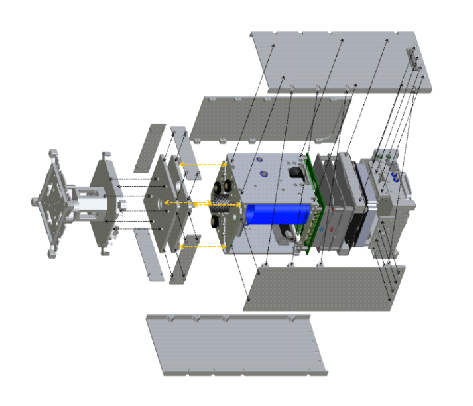
\includegraphics[width=0.6\textwidth]{02/fig/2-3-2.eps}
	\caption{組み立て図}
	\label{2-3-2}
\end{figure}

図\ref{2-3-4}に本衛星の通信回線を示す.本衛星はコマンドアップリンクにアマチュアVHF帯,テレメトリダウンリンクにアマチュアUHF帯を用いる.アンテナはいずれも展開式の半波長モノポールアンテナ(特注品のリン青銅製コンベックステープ)を使用する.地上局については既存の東工大局のハードウェアおよびソフトウェアを一部更新して用いた.
さらに,5.84GHz通信を実現するため,FITSAT-1で用いたものと同等の通信機(ロジカルプロダクト社LPTX5840-1,出力2W)を衛星に搭載する.衛星に搭載した5.84GHz円偏波パッチアンテナは購入品では性能が低かったため新規開発し搭載した.地上局については,FITSAT-1で用いたのと同等のLNB (Low Noise Block Converter)を購入し,東京工業大学が保有していたパラボラアンテナに設置した.これにより,アマチュア5.8GHz帯で最大115kbpsの通信を行う.パッチアンテナはバス部の端面に取り付けられる.本アンテナは半値幅約60 degの指向性であり,これを地上へ向ける姿勢制御が必要である.本衛星では,FITSAT-1にて実績のある,永久磁石を用いた沿磁力線姿勢制御を行う.角速度のダンピングについては,PCパーマロイの板を用いたヒステリシスダンパにより行う.姿勢制御の概要を図\ref{2-3-5}に示す.
\begin{figure}[H]
	\centering
	\includegraphics[width=0.6\textwidth]{02/fig/2-3-4.jpg}
	\caption{通信回線の概要}
	\label{2-3-4}
\end{figure}
\begin{figure}[H]
	\centering
	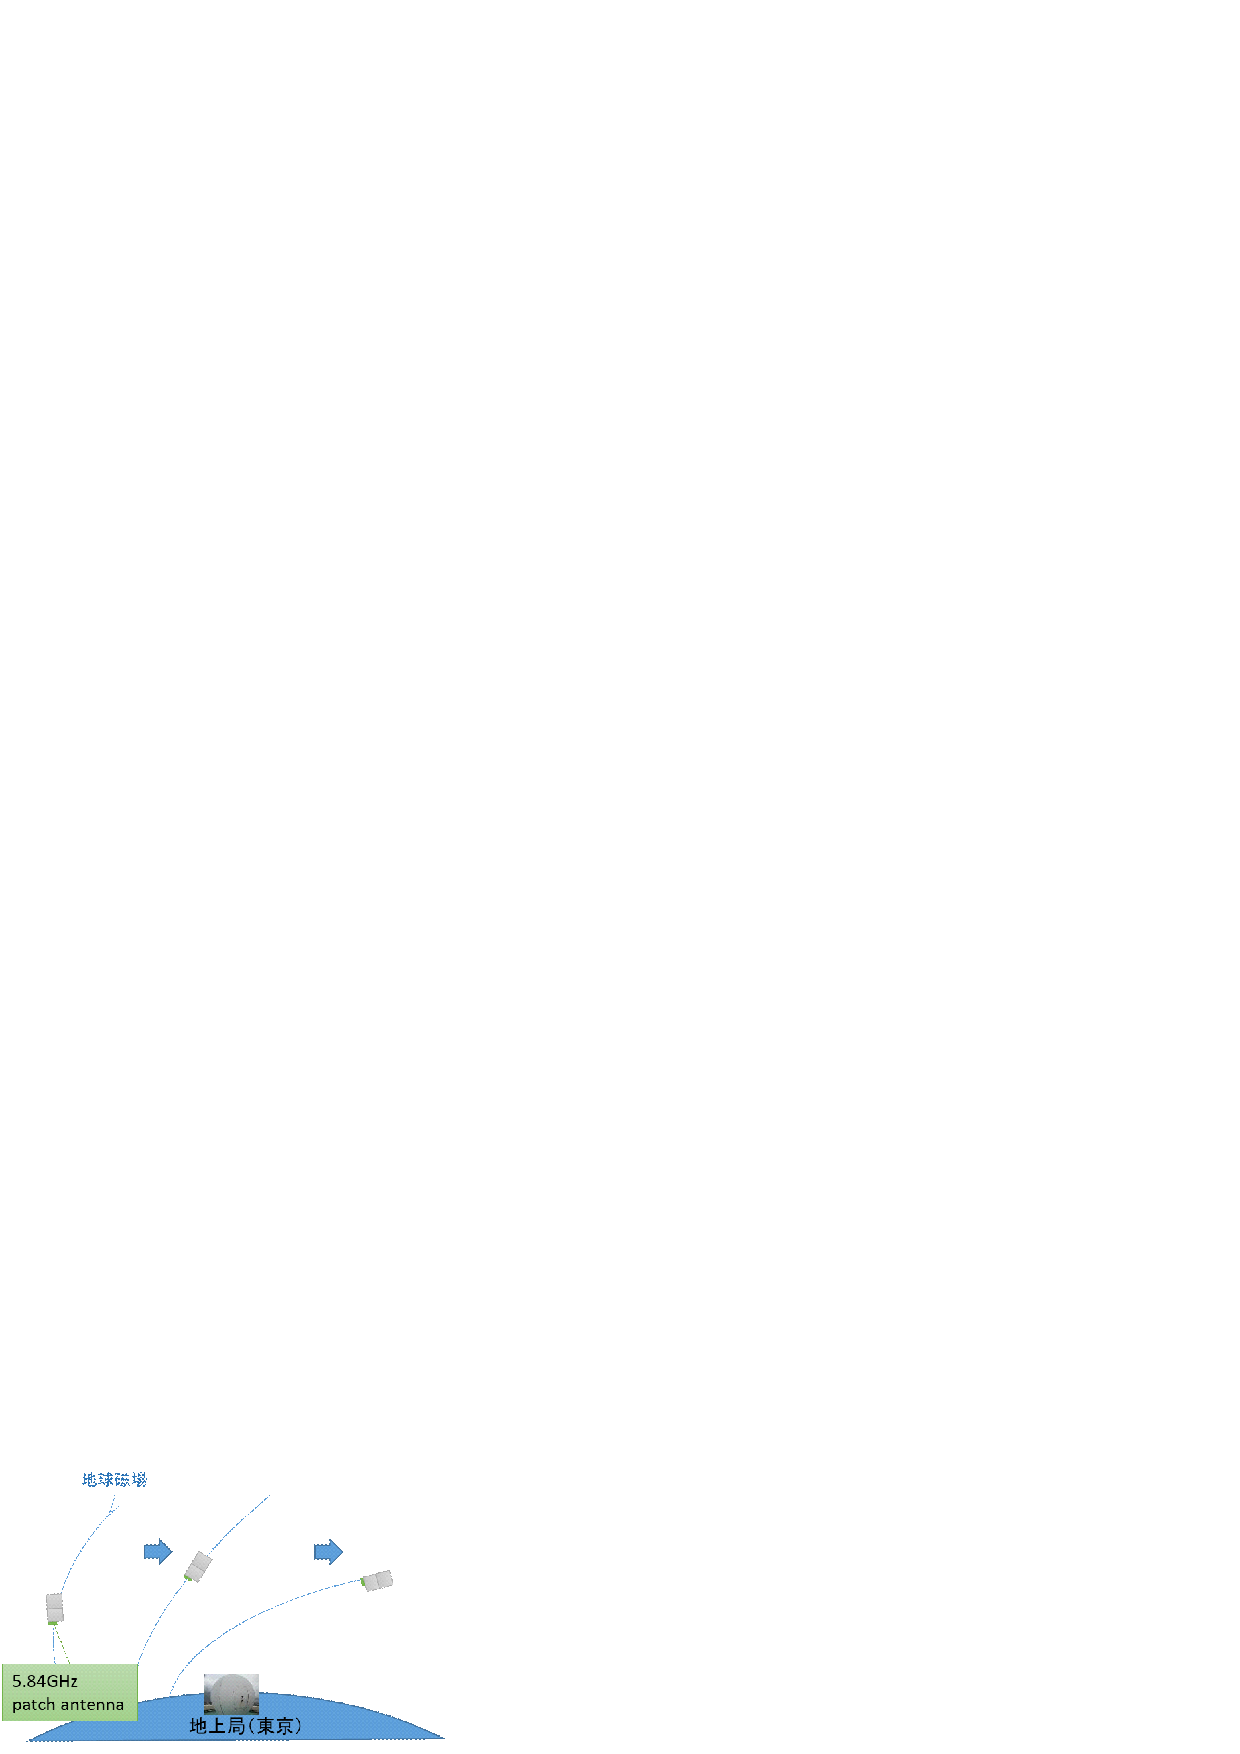
\includegraphics[width=0.5\textwidth]{02/fig/2-3-5.png}
	\caption{永久磁石を用いた沿磁力線制御}
	\label{2-3-5}
\end{figure}

\subsection{システムダイアグラム}
OrigamiSat-1 のシステムダイアグラムを図\ref{2-3-3}に示す.
\begin{figure}[H]
	\centering
	\includegraphics[width=1.0\textwidth]{02/fig/2-3-3.jpg}
	\caption{OrigamiSat-1フライトモデルのシステムダイアグラム}
	\label{2-3-3}
\end{figure}	% 2章 ミッション定義
% 3章
\chapter{サブシステム開発の経緯(設計・試験)}
\label{chap:subsystem}

%********************************
%図の追加
%\begin{figure}[H]
%	\centering
%	\includegraphics[scale=1]{03/fig/3-2-1.jpg}
%	\caption{図の説明文}
%	\label{fig3-2-1}
%\end{figure}
%
%%表の追加
%\begin{table}[H]
%	\centering
%	\includegraphics[scale=1]{03/fig/t3-2-1.jpg}
%	\caption{表の説明}
%	\label{table3-2-1}
%\end{table}
%********************************

\section{電源系 (概要/EPS/インヒビット設計(二重絶縁)/電源系統図/電池/SAP)(池谷・中塚)}
\subsection{概要}
本節では本衛星の電源系について述べる.

本衛星の電源系の概要を
に示す.

電源系統図挿入

本衛星の電源系は主に以下のコンポーネントから構成されている.
\begin{itemize}
	\item 太陽電池パネル(Solar Array Panel, SAP)
	\item 電源基板EPS
	\item バッテリ
	\item インヒビット回路
	\item CIB電源系
	\item ミッション部電源系
\end{itemize}


\begin{landscape}
\begin{figure}[htbp]
	\begin{center}
		\includegraphics[width=0.5\linewidth]{./03/fig/Power_diagram.png}
		\caption{Example of a figure caption.}
		\label{mir}
	\end{center}
\end{figure}
\end{landscape}            


\subsection{SAP}

\subsubsection{SAP試験}

\subsection{バッテリ}


\subsection{CIB電源系}

\subsection{EPS}


\subsection{ミッション部電源系}
\section{通信系 (衛星) (大本)}

本衛星に搭載する通信機としては,以下の3つがある.
\begin{itemize}
	\item {1} 地上局からのアップリンクを受信するVHF系
	\item {2} 地上局へCW信号,FM信号をダウンリンクするUHF系
	\item {3} 地上局へ大容量データをダウンリンクする5.8GHz系
\end{itemize}

衛星と地上局の通信の概略図を図\ref{fig4-2-1}に示す.
本衛星の回線設計は本衛星の軌道情報,東工大松永研究室地上局設備の性能を加味し,図\ref{fig4-2-2}のようになされた.
それぞれに要求される性能を記述する.
\begin{figure}[H]
	\centering
	\includegraphics[scale=0.5]{03/fig/4-2-1.jpg}
	\caption{通信系概略図}
	\label{fig4-2-1}
\end{figure}
\begin{figure}[H]
	\centering
	\includegraphics[scale=0.4]{03/fig/4-2-2.jpg}
	\caption{回線設計}
	\label{fig4-2-2}
\end{figure}

\subsection{VHF系}
VHF帯(Very High Frequency)の通信機では地上局からのアップリンクを受信するために用いる.通信機は西無線研究所の301A型を用いた.
アンテナにはコンベックス加工を行ったリン青銅製のモノポールアンテナ(幅5mm, 厚さ0.1mm)のものを用い,長さはインピーダンスマッチング試験を通じて決定した.
以下に設計スペックおよび系統図(\ref{fig4-2-3})を示す.
\begin{itemize}
	\item 周波数:145.980MHz
	\item 送信出力:100mW(CW),800mW(CW)
	\item 寸法:60x50x10.5mm
	\item 重量:38g
	\item アンテナ利得:0dBi
	\item 周波数帯域幅:500Hz(CW),20kHz(FM)
\end{itemize}
\begin{figure}[H]
	\centering
	\includegraphics[scale=0.6]{03/fig/4-2-3.jpg}
	\caption{UHF/VHF系通信系統図}
	\label{fig4-2-3}
\end{figure}

\subsection{UHF系}
UHF帯(Ultra High Frequency)の通信機では地上局へCW信号,FM信号をダウンリンクするために用いる.通信機は西無線研究所の301A型を用いた.
アンテナにはコンベックス加工を行ったリン青銅のモノポールアンテナ(幅5mm, 厚さ0.1mm)のものを用い,長さはインピーダンスマッチング試験を通じて決定した.
以下に設計スペックおよび系統図(\ref{fig4-2-3})を示す.
\begin{itemize}
	\item 周波数:437.505MHz
	\item 寸法:100x60x10.5mm
	\item 重量:60g
	\item アンテナ利得:0dBi
\end{itemize}

\subsection{5.8GHz系}
5.8GHz系の通信機では画像などの大容量データをダウンリンクするために用いる.通信機はロジカルプロダクト社製 LPTX5840-1を用いた.
アンテナには円偏波パッチアンテナ(30x30x1.6mm)を用いた.
以下に設計スペックおよび系統図(\ref{fig4-2-4})を示す.
\begin{itemize}
	\item 周波数:5840MHz
	\item 送信出力:2W
	\item 寸法:76x70x16mm
	\item 重量:220g
	\item アンテナ利得:3dBi
	\item 周波数帯域幅:210kHz
\end{itemize}
\begin{figure}[H]
	\centering
	\includegraphics[scale=0.6]{03/fig/4-2-4.jpg}
	\caption{5.84GHz系通信系統図}
	\label{fig4-2-4}
\end{figure}

\section{地上局(加藤・飯島)}
\section{C\&DH系(OBC 岩崎・小出・林・井手, COBC 黒崎・中塚・大本, Rpi 飯島)}
%ソフトウェア設計思想
%HKデータ
%コマンド予約・実行
%機能確認

%文責:黒崎・小出
%***各項目の執筆担当者名は最後に消してください

\subsection{初期運用}
%画像のファイル名は「3-4-Ini-1.jpg」「3-4-Ini-2.jpg」...
%ラベル名は「fig3-4-Ini-1」「fig3-4-Ini-2」...

\subsubsection{初期運用概要(余裕があれば黒崎.無理なら小出)}
初期運用とは?目的.

\subsubsection{基本設計思想(余裕があれば黒崎.無理なら小出)}
\begin{itemize}
	\item \textbf{OBCがメインで溶断を行う.OBCが溶断に失敗している場合にCIBが溶断を行う.}本来であれば,SavingモードでOBCの電源が切られてしまうため,CIBがメインで溶断を行いたかったが,CIBは初期運用以外の開発がかなり遅れていたため,初期運用のデバックに割ける時間が限られておりOBCをメインにしたという背景がある.
	\item \textbf{溶断頻度は22.5分間隔.}これは地球1周を90分かけるOrigamiSat-1の軌道において,地球1周の間に4回溶断をトライする設計になっている.地球1周分を基準に考えているのは,日向,日陰条件で宇宙環境温度が異なり,溶断の成功確率に影響が出ることを考慮している.
	\item \textbf{1日の間で8回(地球2周分)溶断をトライした後は,溶断を行わず待機.}これはバッテリーを温存するためである.
\end{itemize}

\subsubsection{開発の流れ(余裕があれば黒崎.無理なら小出)}
FM試験項目表作成→フローチャート作成→話し合い→フローチャート修正→ソフト書く→デバック→フローチャートとソフトが対応しているか確認→OBC/CIB統合→恒温槽試験で溶断時間の確認→FMで最終確認

\begin{figure}[H]
	\centering
	\includegraphics[scale=0.8,angle=90]{03/fig/3-4-Ini-1.pdf}
	\caption{OBCシート}
	\label{fig3-4-Ini-1}
\end{figure}

\subsubsection{OBC初期運用モードソフト詳細(小出)}
フローチャート的なものとセットで

\subsubsection{CIB初期運用モードソフト詳細(黒崎)}
フローチャート的なものとセットで

\subsubsection{初期運用 運用結果(余裕があれば黒崎.無理なら小出)}
CW HKデータで溶断済みを確認

\subsubsection{コメントや次回の改善点}
\hspace{2ex}
\textbf{OBC / CIB共通(黒崎・小出)}
\begin{itemize}
	\item 溶断済みフラグをCW HKデータのフリースペースの1byteに入れたのは神采配だったと思う.OrigamiSat-1の場合,アップリンクでEEPROMの指定アドレスを読んでダウンリンクする機能が使えなくなってしまっていたため,CW HKデータ以外に溶断済みを確認する術が無かった.
	\item OBCとCIBが同時に溶断を行ってしまった場合,バッテリーがどの程度減少するかの検証をできていなかった.
	\item OBCとCIBのどちらが,何回目の溶断で溶断を成功し,ダウンリンクを開始したかを分かるようにした方がいいのかもしれない.
\end{itemize}

\hspace{2ex}
\textbf{OBC(小出)}
\begin{itemize}
	\item aaaaaaaa
\end{itemize}

\hspace{2ex}
\textbf{CIB(黒崎)}
\begin{itemize}
	\item aaaaaaaa
\end{itemize} %初期運用
\section{姿勢制御系}

\subsection{制御方式}
OrigamiSat-1 搭載の 5.8GHz 通信用パッチアンテナは指向性を持つため,同アン
テナ取付面を地上に向ける姿勢制御が必要となる.本衛星では,永久磁石と地
磁気の干渉を利用した受動的姿勢制御を採用した.飛行と姿勢のイメージを図
\ref{image_attitude_ctrl}に示す.衛星内部に搭載された棒磁石により姿勢
は地磁場の磁力線に沿う様に回転する.この過程で,日本の緯度付近を通過す
る際,パッチアンテナの面が地上を向く.但し,軌道上では運動を減衰させる
要素が乏しく,実際には磁力線を中心に揺動運動することとなる.このため,
本衛星では,PCパーマロイ製のヒステリシスダンパを搭載している.本ダンパ
は,磁力線の相対運動に伴い電磁誘導を生じ,内部抵抗による電力消費によっ
て,運動を熱に変換する.本方式は,同じく5.8GHzパッチアンテナを搭載して
いた,FITSAT-1(にわか)に採用され,実績があることから採用した.

\begin{figure}[htbp]
	\centering
	\includegraphics[width=10cm]{./03/fig/image_attitude_ctrl.png}
	\caption{飛行と姿勢のイメージ}
	\label{image_attitude_ctrl}
\end{figure}

\subsection{主要諸元}
本衛星の姿勢制御用永久磁石およびヒステリシスダンパの搭載イメージを図
\ref{image_mag_HD}に示す.また,それぞれの諸元を表
\ref{spec_magnet}, 表\ref{spec_HD}に示す.

\begin{figure}[htbp]
	\centering
	\includegraphics[width=5cm]{./03/fig/image_mag_HD.png}
	\caption{永久磁石とヒステリシスダンパ搭載イメージ}
	\label{image_mag_HD}
\end{figure}

\begin{table}[htb]
    \centering
    \caption{OrigamiSat-1搭載磁石諸元}
    \label{spec_magnet}
    \begin{tabular}{cc} \hline
      項目 & 諸元 \\ \hline\hline
      材質 & Nd \\
        体積 & $2.73 \times 10^{-6} [\rm{m^3}]$\\ 
        磁束密度 & 0.468 [T] \\ 
        発生トルクオーダー & $10^{-5}$ [Nm] \\ \hline   
    \end{tabular}
    \label{requirment_op}
\end{table}

\begin{table}[htb]
    \centering
    \caption{OrigamiSat-1 搭載ヒステリシスダンパ諸元}
    \label{spec_HD}
    \begin{tabular}{cc} \hline
      項目 & 諸元 \\ \hline\hline
        材質 & PC パーマロイ \\
        体積(X-axis) & 1.603 $\times 10^{-7} [\rm{m^3}]$ \\
        体積(Y-axis) & 1.320 $\times 10^{-7} [\rm{m^3}]$ \\
        体積(Z-axis) & 5.055 $\times 10^{-8} [\rm{m^3}]$ \\
        飽和磁束密度 & 0.65 [T] \\
        残留磁束密度 & 0.40 [T] \\
        保磁力 & 1.2 [A/m] \\
        発生トルクオーダー & $10^{-6}$ [Nm] \\ \hline    
    \end{tabular}
    \label{requirment_op}
\end{table}

\subsection{姿勢解析}
衛星の回転運動に関する運動方程式は,次式で表される.
\begin{equation}
  \bm{I} \dot{\bm{\omega}} + \bm{\omega} \times \bm{I} \bm{\omega} = \bm{T}
\end{equation}

ここで,$\bm{I}$は慣性テンソル,$\bm{\omega}$は角速度,$\bm{T}$は外力
トルクである.本衛星では,地磁気と永久磁石による磁気トルク $\bm{T}_{m}$,
地磁気とヒステリシスダンパによる磁気トルク $\bm{T}_{d}$,空気抵抗によるトルク
$\bm{T}_{air}$,太陽光輻射圧トルク $\bm{T}_{sun}$,重力傾斜トルク
$\bm{T}_{g}$ を想定し,$\bm{T}$ を式\ref{3_5_torque}で与える.
\begin{equation}
  \bm{T} = \bm{T}_{m} + \bm{T}_h + \bm{T}_{sun} + \bm{T}_{air} + \bm{T}_{g} \label{3_5_torque}
\end{equation}

\subsubsection{磁気トルク}
地磁気と衛星搭載磁石により発生するトルクは,磁石の磁気モーメント
$\bm{M}_m$ と 地球磁場 $\bm{H}$ により次式で表される.
\begin{eqnarray}
  \bm{T}_{m} = \bm{M}_{m} \times \bm{H} \\
  \bm{M}_m = \frac{V_m}{\mu_0} \bm{B_m}
\end{eqnarray}
ここで,$V_m$は磁石の体積, $\mu_0$は真空の透磁率,$\bm{B_m}$は磁石の
磁束密度ベクトルである.

\subsubsection{ヒステリシスダンパ}
常磁性体は外部磁場により磁化された後,図\ref{3_5_hysteresis_loop}に示
すように,外部磁場が減少し0になっても,磁化(磁束密度)が残留する(ヒス
  テリシスを持つ).このヒステリシスループを巡る過程でエネルギー損失が
発生し,ダンパとして作用する.

\begin{figure}[htbp]
	\centering
	\includegraphics[width=8cm]{./03/fig/3_5_hysteresis_loop.jpg}
	\caption{磁性体のヒステリシス}
	\label{3_5_hysteresis_loop}
\end{figure}

ヒステリシスダンパの磁束密度$B_h$は,地球磁場により次式のように与えられる.
\begin{equation}
B_h = \frac{2B_s}{\pi}\tan^{-1}\left[\frac{1}{H_0}\tan\left(\frac{\pi
    B_0}{2B_s}\right)(H \pm H_0) \right]
\end{equation}
ここで,$B_s$, $B_0$, $H_0$ はそれぞれヒステリシスダンパの飽和磁束密度,
残留磁束密度,保持力である.
この時,ヒステリシスダンパトルク$\bm{T}_h$は,
\begin{eqnarray}
  \bm{T}_{h} = \bm{M}_{h} \times \bm{H} \\
  \bm{M}_h = \frac{V_h}{\mu_0} \bm{B_h}
\end{eqnarray}
となる.ここで $\bm{M}_h$,$V_h$は,それぞれヒステリシスダンパの磁気モー
メント,体積である.
永久磁石とヒステリシスダンパのサイジングについては,後述のシミュレーション結果に基づく
遺伝的アルゴリズムにより決定した.

\subsubsection{太陽光輻射トルク}
光圧は,鏡面反射,拡散反射,吸収によって異なり,それぞれの単位面積当た
りの光圧 $d \bm{f}_a$, $d \bm{f}_s$, $d \bm{f}_d$, はそれぞれ次式で表
される.
\begin{eqnarray}
  d \bm{f}_a &=& -M_s\rho_a(\bm{s} \cdot \bm{n})\bm{s}dA  \\
  d \bm{f}_s &=& -2M_s\rho_s (\bm{s} \cdot \bm{n})^2
  \bm{n}dA \\
  d \bm{f}_d &=& -M_s\rho_d (\bm{s} \cdot \bm{n}) \left(\bm{s} +
  \frac{2}{3}\bm{n} \right) dA
\end{eqnarray}
ここで,$\rho_a$, $\rho_s$, $\rho_d$ はそれぞれ,光の吸収率,鏡面反射
率,拡散反射率であり,光が透過しない材料では以下の関係を持つ.
\begin{equation}
  \rho_a + \rho_s + \rho_d = 1
\end{equation}
また,$\bm{s}$は太陽方向ベクトル, $\bm{n}$は衛星表面の法線ベクトル,
$A$は照射面積である.
$M_s$ は,次式で定義される.
\begin{equation}
  M_s = \frac{E_s}{c} \cdot \left( \frac{AU}{r_{sun}} \right)^2
\end{equation}
ここで,$E_s$, $c$, $AU$, $r_{sun}$はそれぞれ,太陽定数,光速,地球-太
陽間距離,衛星-太陽間距離である.
これらを用いて,太陽光輻射圧トルクは次式で与えられる.
\begin{equation}
  \bm{T}_{sun} = \int_{\bm{s}\cdot\bm{n}} \bm{r} \times \nu(d\bm{f}_a +
  d\bm{f}_s + d\bm{f}_d)
\end{equation}
ここで $\nu$ は日照条件である.(日照: $\nu=1$, 日陰: $\nu=0$).


\subsubsection{空気抵抗トルク}
空気抵抗トルクは次式で与えられる
\begin{equation}
  \bm{T}_{air} = \int_{\bm{n}\cdot\bm{v}} \bm{r} \times
  -\frac{1}{2}C_d\rho (\bm{n}\cdot\bm{v})\bm{v} dA
\end{equation}
ここで,$\bm{r}$は衛星重心から空力中心への位置ベクトル,$C_d$ は空気抵
抗係数,$\rho$ は大気密度,$\bm{v}$ は衛星の速度ベクトルである.

\subsubsection{重力傾斜トルク}
重力傾斜トルクは,次式で与えられる.
\begin{equation}
  \bm{T}_g = -\frac{3\mu}{|\bm{r_e}|^3}\bm{r_e} \times (\bm{I} \cdot
  \bm{r_e})
\end{equation}
ここで,$\mu$は地球重力定位数,$\bm{r_e}|$は地球重心から衛星重心への位
置ベクトル,$\bm{I}$は衛星の慣性テンソルである.

\subsection{解析結果}
上記の式に基づき,地球周回時の OrigamiSat-1 の姿勢についてシミュレーショ
ンを行った.地球磁場については,国際地球電磁気学会の標準磁場モデルであ
る IGRF (International Geomagnetic Reference Field) を用いた.
また,大気モデルとして Harris Priester Model を用いた.

以下,各条件におけるOrigamiSat-1の運動予測について結果を示す.
各軸方向は,図\ref{image_mag_HD}の通りである.

\subsubsection{3U 膜展開前}
E-SSODより放出された直後を想定し,3U状態,膜面未展開,マスト伸展無し,
高度500km,初期角速度が全軸 0 という条件における角速度および,
機体z軸と地球磁力線とのなす角をそれぞれ図\ref{3_5_sim_3udep_angvel}と
図\ref{3_5_sim_3udep_zang}に示す.放出からおよそ16000秒程度で姿勢が安
定している.

\begin{figure}[htbp]
	\centering
	\includegraphics[width=9cm]{./03/fig/3_5_sim_3udep_angvel.png}
	\caption{放出直後の角速度推移(初期角速度無し)}
	\label{3_5_sim_3udep_angvel}
%\end{figure}
%\begin{figure}[htbp]
	\centering
	\includegraphics[width=9cm]{./03/fig/3_5_sim_3udep_zang.png}
	\caption{放出直後の機体z軸と地球磁場のなす角度の推移 (初期角速
          度無し)}
	\label{3_5_sim_3udep_angvel}
\end{figure}

また,初期角速度を,x軸: 30deg/s, y軸: 30deg/s, z軸: 5deg/s,とした場
合についての結果を図\ref{3_5_sim_3udep_angvel2}と
図\ref{3_5_sim_3udep_zang2}に示す.この条件においても,静定に数日を要
するものの,姿勢は静定する.

\begin{figure}[htbp]
	\centering
	\includegraphics[width=9cm]{./03/fig/3_5_sim_3udep_angvel2.png}
	\caption{放出直後の角速度推移 (初期角速度あり)}
	\label{3_5_sim_3udep_angvel2}
%\end{figure}
%\begin{figure}[htbp]
	\centering
	\includegraphics[width=9cm]{./03/fig/3_5_sim_3udep_zang2.png}
	\caption{放出直後の機体z軸と地球磁場のなす角度の推移 (初期角速
          度あり)}
	\label{3_5_sim_3udep_angvel2}
\end{figure}

\subsubsection{2U 膜切り離し後}
ミッションの後半.マストおよび膜切り離し後に2U状態となった際の運動につ
いて,機体の慣性条件が変化しても姿勢安定が成立するかを検討した.2U状態,高度400km,初期角速度が全軸 0 という条件における角速度および,
機体z軸と地球磁力線とのなす角をそれぞれ図\ref{3_5_sim_2u_angvel}と
図\ref{3_5_sim_2u_zang}に示す.2Uの状態においても,放出からおよそ10000秒程度で姿勢が安
定している.

\begin{figure}[htbp]
	\centering
	\includegraphics[width=9cm]{./03/fig/3_5_sim_2u_angvel.png}
	\caption{膜切り離し後の角速度推移}
	\label{3_5_sim_2u_angvel}
%\end{figure}
%\begin{figure}[htbp]
	\centering
	\includegraphics[width=9cm]{./03/fig/3_5_sim_2u_zang.png}
	\caption{膜切り離し後の機体z軸と地球磁場のなす角度の推移}
	\label{3_5_sim_2u_zang}
\end{figure}

\subsubsection{3U 膜展開時}
膜展開状態は,空力,太陽光輻射,重力傾斜各トルクの外乱が大きくなること
が予想されるが,この状態おいても姿勢安定が可能であれば,5.8GHz高速通信
が可能となる.3U状態,高度500km,マスト伸展状態,初期角速度が全軸 0 という条件における角速度および,機体z軸と地球磁力線とのなす角をそれぞれ図\ref{3_5_sim_membrane_angvel}と
図\ref{3_5_sim_membrane_zang}に示す.こちらは角速度が発散することは無
く,$10^{-1}$deg/sオーダーの運動となっているが,姿勢は安定せず5.8GHzパッ
チアンテナを地上に向け続けることは困難であることが判明した.本結果に基
づき,5.8GHz高速通信については膜切り離し後に実施することとし,それまで
大容量の実験データは機体上に保存しておくこととした.

\begin{figure}[htbp]
	\centering
	\includegraphics[width=9cm]{./03/fig/3_5_sim_membrane_angvel.png}
	\caption{膜展開時の角速度推移}
	\label{3_5_sim_membrane_angvel}
%\end{figure}
%\begin{figure}[htbp]
	\centering
	\includegraphics[width=9cm]{./03/fig/3_5_sim_membrane_zang.png}
	\caption{膜展開時の機体z軸と地球磁場のなす角度の推移}
	\label{3_5_sim_membrane_zang}
\end{figure}

\section{構体系(奥山・大野) 重量管理も含む}

\if0
奥山
・工場の人と仲良くして納期短縮
・放出検知ピン(二硫化モリブデン,PEEK)
・基板保持ねじれ
・EMの不具合
・基板保持の治具
・精度出しの方法どうやって決めたか
・組立手順どう決めたか
・発注
・サーミスタ
・配線

ひらくさん
・組み立て精度が出せない(組み立てが異常に複雑)
・レールの長さが足りなかった →形状計測
・レールの粗さ計測を実施していなかった →形状計測
・ハードアノダイズ処理の2度手間が生じた(納期長い)
・FMでのディプロメントスイッチ不具合
・FM振動試験時、配線を噛んでしまっていた
  
  ----------------------------------------
  CAD作成
  ・干渉チェック
  ピッタリは危険(展開アンテナはまったやつ)
  ・EMの不具合:FM発注リスト参照
  ・CAD非反映物(ハーネス、コネクタ等)の考慮
  ・ハーネスの通り道にR
  ・ディプロイメントスイッチななめる
  ・工具が入るか パッチ土台とか
  
  図面作成
  ・加工時見やすいように
  ・公差の指定
  ・加工順序考える
  ・早めに工場と相談
  
  発注
  ・業者と工場の違い
  ・納期注意
  ・誰が見ても誤解しない図面
  ・アルマイト時間かかる マスキングとか
  
  
  加工
  ・ハードアノダイズ処理の2度手間が生じた(納期長い)
  ・基板保持ねじれ 組み立て?
  
  組み立て
  ・基板保持の治具
  ・基板入ったりはいらなかったり、、
  ・サーミスタ
  ・FM振動試験時、配線を噛んでしまっていた
  ・配線
  ・精度出しの方法どうやって決めたか
  ・組立手順どう決めたか
  ・組み立て精度が出せない(組み立てが異常に複雑)
  ・FMでのディプロメントスイッチ不具合
  ・手順書 誰でも組み立てられるように
  とくにバスはソフトの人もできるようにしておくべき
  全工程ソフトの人と確認
  ・工具は毎回しまう
  
\fi

本稿では,私が携わったEMの設計の修正からFMの組立までについて,各開発フェーズごとに記載する.
なお,詳細な不具合は「OP-S1-0065\_OrigamiSat-1不具合・A/I管理表\_20190124」に記載している.また,設計についてEMからFMで修正する際の修正項目(EMでの不具合項目)は「FM発注リスト.xlsx」に記載している.


\subsection{3DCAD設計}
3DCAD設計でミスが起こると開発が進んだときの手戻りが大きいので気をつける.
\subsubsection{干渉の確認}
構体の部品同士の干渉を確認する必要がある.ここで注意したいことが,加工公差である.CAD上では公差は指定していないため,公差を含めて干渉がないかを考慮する必要がある.EMでは,展開アンテナとそれを通す溝の幅が同じであったため,CAD上では干渉はないが,実際にはアンテナがはまって展開できなかった.(追加工で対応)
\subsubsection{ハーネス・コネクタ等の電子部品の考慮}
CADでハーネス,コネクタを入れることをお勧めする.ハーネスがどこを通るか,通る場所には通れるだけの隙間があるか,コネクタは干渉しないかを確認する必要がある.また,ハーネスは曲率の限界があるので注意する.
\subsubsection{ハーネスの通り道に突起物を置かない}
特に注意するのが,構造部品の角である.振動等でハーネスの皮膜が破れる恐れがあるため,Rをつける.また,さらに補強としてハーネスにガラスクロステープを巻いた.
\subsubsection{組立を考慮した設計}
組み立てについては,工具の大きさと,組み立てのしやすさを考慮する必要がある.工具の大きさについては,組み立て時に工具と部品に干渉なく組み立てられるかを注意する.底面パネルに対するパッチアンテナ土台の取り付けは,取り付けるねじに対して工具を同軸で取り付けるべきであるが,底面パネルと工具が干渉するので,工具を斜めにして取り付けていた.組み立てのしやすさについては,D-subの取り付け等無理な体勢での組み立てがあったので,良くない.何度かワッシャを構体内に落としたこともあったので注意して欲しい.
\subsubsection{ばか穴による組み立てのズレの考慮}
ばか穴にしている箇所は,ねじの径との差の範囲で部品間が相対的にずれる.0.1mmオーダーの差があり,レール精度は±0.1mmであるので,十分影響がある.要求精度以外にも,ディプロイメントスイッチの接触不良があった.スイッチの位置によってディプロイメントピンとの相対的位置関係が変わり,スイッチ起動の要求,インターフェイスを満たせない場合があった.今回はスイッチ取り付け後のピンを取り付ける際に位置を調整することで対処した.


\subsection{図面作成}
図面作成は寸法を全て書き込めば良いだけでなく,加工する際に必要な寸法を書くことが重要である.自ら加工することも少なくなかったので,そのような経験があるとよりうまく書けると思う.
%%\subsubsection{加工者への考慮}

%%\subsubsection{公差の指定}
\subsubsection{加工順序の考慮}
自分で加工するとき,前日までに加工順序を確認しておくことをお勧めする.当日朝から工場に行ってから工程を考えると進捗が得られない.
\subsubsection{加工者との早めの相談}
公差等わからないことがあったら専門家に聞くほうが良い.考えるより細かい部分は話しながら決めたほうが早く進む.


\subsection{発注}
発注は相手に誤解されないように伝えることが重要である.
\subsubsection{業者と工場の違い}
基本的には工場の発注が良い.工場のメリットは大学内に併設しているので直接コンタクトがとりやすい.外部業者であるとメールのみのやり取りで伝えきれないことがあったりする.外部業者は,工場が立て込んでいて納期が遅かったり,休業のときに利用する.工場は大学内の様々な案件を行っているので,時期によっては納期がだいぶ先になる.また,外部業者で工場が海外であると日本と休日が異なるため,助かることがある.(特にGW)
%%\subsubsection{納期の考慮}


\subsection{組み立て}

\subsubsection{手順の決め方}
基本的には底面パネルから膜展開部に向かって組み立てる.それに加え,左記の流れであると組めない部分は順序を適宜変えた.また,レール精度が求められている部品(底面パネル,側面パネル×4,膜展開部)に関してはトルクはかけずに仮締めを行い,その後精度出しを行った.最終的な手順は「組み立て手順書」に記載する.
\subsubsection{手順書の作り方}
誰でも組み立てができることを目標とした.組み立て時に考えることはないようにする.また,ソフトを書く人にはバス系の組立ができるようにしてもらうことを薦める.ソフトを書き込むために分解が必要なときもあるので,そのたびに構体系の担当がいないと開発が進まない事態になったことが何度もあった.
\subsubsection{精度出しの方法}
精度出しの方法は「組み立て手順書」に記載している.
\subsubsection{基板保持の冶具}
基板保持とCIBの取り付け誤差により,基板がずれて側面パネルが固定できないことが何度かあった.それにより,基板保持とCIBの相対位置を固定する冶具を作成した.
\subsubsection{基板の組み立て誤差}
上記の対応で精度は良くなったが,その先の基板を取り付けた際に再現性がなく,側面パネルと干渉することがあった.これの原因はわかっていない.
\subsubsection{サーミスタの貼付方法}
サーミスタを貼り付ける際は貼り付ける部品にカプトンテープを貼り,その上にサーミスタを置き,上からカプトンテープを貼る.このとき,どちらのカプトンテープも多数の穴を開けた.これは,真空中でカプトンと部品との間の気泡が膨張し,カプトンがはがれることを防ぐためである.
\subsubsection{配線}
ハーネスの経路は,構体部品との干渉を避けることとハーネスの可動域を考慮してどのように動いても 部品間でハーネスをはさまないよう取り回すことを考慮する.後者についてはFMの1回目の振動試験でハーネスを構体部品ではさんでしまっていたので,はさんでしまったハーネスを別のハーネスをくぐらせて動いたとしても挟まれないようにした.
\subsubsection{ディプロイメントスイッチの不具合}
ディプロイメントピンの公差の指定を誤り,底面パネルにピンが固着してしまった.対策としては,底面パネルの穴を削り,微調整した.また,ピンには二硫化モリブデン処理を施し,摩擦係数を減らした.
\subsubsection{工具の管理}
工具は作業が終わっていなくてもその日中には片付けることを徹底する.放置したり,他の人が使ったりした後,翌日に探すことが多々あった.構体系のみならず開発者全員の認識が必要である.



\section{熱系(中村・坂本)}

\subsection{熱設計の方針}
熱系については,下記の考え方のもと設計・検証を実施した.この考え方は主に,戸谷剛・北海道大学准教授がふくい宇宙産業創出研究会WGで講演(2016年11月24日)された資料をご厚意で見せていただき,そこからの学びを元に構築した.
\begin{itemize}
	\item 温度が均一化できるところをなるべく増やし,複雑度を下げる方針とした.
	\item Thermal Desktop等解析ソフトを用いた詳細解析は行わず,解析については少数節点解析でのパラメータサーベイのみを行った.結果,当初設計の表面仕上げで良いとの見込みのもと開発を進めた.
	\item 受動的熱制御を主体とした.ただし,開発の最後のフェーズでバッテリにヒータを貼付し,能動的熱制御を取り入れる設計変更をした.
	\item 材料の熱光学パラメータは宇宙科学研究所小川研のご厚意で,TESA2000を使用させていただき計測した.
	\item 接触コンダクタンスの影響を少なくするため熱伝導シートを導入した.
	\item ウェルリサーチ社の熱真空槽を用い,熱平衡試験でパラメータ同定をしたのちに,熱真空試験で機器の動作確認をした.これらの試験については別章に記載する.
\end{itemize}

下図のように節点へ分割したモデルを作成した.Matlabを用いin-houseでプログラムを書いた.
\begin{figure}[H]
	\centering
	\includegraphics[width=0.8\textwidth]{03/fig/3-7-1.jpg}
	\caption{節点法による熱解析}
	\label{fig3-7-1}
\end{figure}

パラメータ同定のために熱平衡試験を実施した.試験については別章にて詳説する.概要を数に示す.
\begin{figure}[H]
	\centering
	\includegraphics[width=0.8\textwidth]{03/fig/3-7-2.jpg}
	\caption{熱平衡試験による解析モデルコリレーション}
	\label{fig3-7-2}
\end{figure}
ここで得たパラメータを元に,節点解析モデルを用いて,軌道上での各節点の温度変化を予測した.

\subsection{熱解析結果:高温ケース}
高温ケースで以下の結果を得た.
\begin{figure}[H]
	\centering
	\includegraphics[width=0.5\textwidth]{03/fig/3-7-3.jpg}
	\includegraphics[width=0.5\textwidth]{03/fig/3-7-4.jpg}
	\includegraphics[width=0.5\textwidth]{03/fig/3-7-5.jpg}
	\caption{節点法熱解析結果:高温ケース}
	\label{fig3-7-3}
\end{figure}

\subsection{熱解析結果:低温ケース(Nominal)}
膜展開前の低温ケースで以下の結果を得た.
\begin{figure}[H]
	\centering
	\includegraphics[width=0.8\textwidth]{03/fig/3-7-6.jpg}
	\includegraphics[width=0.8\textwidth]{03/fig/3-7-7.jpg}
	\caption{節点法熱解析結果:低温ケース(Nominal)}
	\label{fig3-7-6}
\end{figure}

\subsection{熱解析結果:低温ケース(膜展開後)}
膜展開後の低温ケースで以下の結果を得た.
\begin{figure}[H]
	\centering
	\includegraphics[width=0.8\textwidth]{03/fig/3-7-8.jpg}
	\includegraphics[width=0.8\textwidth]{03/fig/3-7-9.jpg}
	\caption{節点法熱解析結果:低温ケース(膜展開後)}
	\label{fig3-7-8}
\end{figure}

\subsection{熱系の振り返り}
別章に掲載する軌道上温度のHKデータを見ると,解析結果よりも温度が高く,また温度変化の幅も小さい.したがって解析・実験による予測が適切でなかった可能性がある.
軌道上結果を見る限りでは,バッテリにヒータを追加する設計変更は不要だった可能性がある(ただし膜を展開していないので膜展開時についてはさらなる詳細解析を要する).
\section{VHF/UHF展開アンテナ(仁尾・坂本)}



\section{ミッション系}

OrigamiSat-1は,ミッション系ペイロードとして,以下の3つを有する.本節ではそれぞれの設計と試験について述べる.
\begin{itemize}
	\item 5.8GHz通信ミッション
	\item 伸展カメラミッション
	\item 膜展開ミッション
\end{itemize}

\subsection{5.8GHz通信ミッション(井手)}
ここでは5.84GHz帯高速通信を担うモジュール(以下5.8)について述べる.
\subsubsection{ミッション内容}
衛星内部で膜展開前後の写真・動画を地上局に送る.モジュールは福岡にあるロジカルプロダクト社から購入しており,これは福岡工業大学の衛星プロジェクトで用いたものと同じである.

\subsubsection{ハードの概要}
5.8にはMicrochip Technology社のPIC16F886(以下PIC)を用いており,写真保存用のフラッシュメモリ(以下FROM)はMicron Technology社のM25P32を用いている.ここに回路図の写真.

\subsubsection{ソフトの概要}
PICのプログラムにはC言語を用いている.衛星にはブランチ名master-debugger,コミット番号51237d7e783d32032fe3db0332d3c69a6ab9e13eを書き込んだ.ソフトは1つのメイン文が繰り返し実行されるが,主に2つの部分に分かれている.1つはコマンドをOBCから受け取る部分,もう1つは受け取ったコマンドを実行する部分である.

まずコマンドの受け取り方法について記述する.コマンドはいつOBCから送られてくるかわからないため常に待機状態にあり,CRC16を用いたコマンドのチェックを通過したコマンドのみ実行する.OBCとの通信にはUARTを用いた.通信速度はモジュールの振動子から14400, 57600, 115200[bps]と設定できるが,デフォルトは115200に設定してある.OBCとの通信時には常に115200を用い,地上局との通信時には通信速度を変更することができる.
\subsection{伸展カメラ}
\subsubsection{システム開発(ウェルリサーチ・坂本)}

伸展カメラ部については,週に1回のSkype定例会合を東工大とウェルリサーチで持ち,主に
\begin{itemize}
	\item ハードウェア開発,およびRaspberry Piの基本ソフトの開発まではウェルリサーチが担当.
	\item カメラのキャリブレーションや計測アルゴリズムの開発,およびRaspberry Piの詳細なソフトウェアプログラムを東工大が担当.
\end{itemize}
と共同で実施した.試験はウェルリサーチと東工大坂本研,および古谷研において実施した.
%
開発したシステムについてはウェルリサーチが作成した以下の文書に良くまとまっている.
\begin{itemize}
	\item OS1-TEC-003 設計仕様書
	\item OS1-TEC-005 BBM試験報告書
	\item OS1-TEC-011 放射線試験計画書
	\item OS1-TEC-012 放射線試験報告書
\end{itemize}
本項の以下ではシステムの概要を述べる.実施した試験については次項で述べる.

OrigamiSat-1 に搭載する伸展カメラ部は、(i) 1m の長さの伸展マスト(双安定性 STEM (Storable Tubular Extendable Member))を伸展すること、(ii) 膜展開過程の動画撮影を行うこと、(iii) 膜展張形状のステレオ撮影を行うこと、を担う。
さらに、ミッションシークエンスに示した通り、(iv) 膜展開ミッションの終了後に、膜展開部を切り離すこと、を実施する。システムの主な構成要素を図\ref{fig3-9-2-1-1}に示す。図\ref{fig3-9-2-1-2}にEM 品の写真を示す。図\ref{fig3-9-2-1-3}にSTEMおよびそれに沿ったハーネスを伸展し、切り離す機構の説明を示す。

\begin{figure}[H]
	\centering
	\includegraphics[width=.8\textwidth]{03/fig/3-9-2-1-1.jpg}
	\caption{伸展カメラ部の構成}
	\label{fig3-9-2-1-1}
\end{figure}
\begin{figure}[H]
	\centering
	\includegraphics[width=.4\textwidth]{03/fig/3-9-2-1-2.jpg}
	\caption{伸展カメラ部EM}
	\label{fig3-9-2-1-2}
\end{figure}
\begin{figure}[H]
	\centering
	\includegraphics[width=.8\textwidth]{03/fig/3-9-2-1-3.jpg}
	\caption{伸展マストとハーネスの伸展と切り離し}
	\label{fig3-9-2-1-3}
\end{figure}


\newpage
\subsubsection{三次元計測(飯島・黒崎)}
三次元計測システムの処理は大きく分けて以下のような3つの工程に分けられる.
\begin{itemize}
	\item[工程A.] カメラキャリブレーション(処理1,処理2)
	\item[工程B.] 測定対象の撮影(処理3)
	\item[工程C.] 画像処理(処理4$\sim$処理8)
\end{itemize}

三次元計測システムのフローチャートを図\ref{fig3-9-2-2-1}に示す.図\ref{fig3-9-2-2-1}中では,黒色の四角マークが「処理」,青色のデータマークが「各処理によって作成されたデータ」を示している.

三次元計測システムは処理1から処理9までの計9処理で行われる.(工程A)カメラのキャリブレーションが処理1,処理2,(工程B)撮影対象の撮影が処理3,(工程C)画像処理が処理4から処理8に対応している.

\vspace{2ex}
工程Aで作成されるデータ(レンズパラメータ,ステレオパラメータ)はカメラの設計値に依存する固有値である.すなわち,2度目以降の測定では,工程Aは省略でき,工程B(処理3. 計測対象撮影)以降のみを行えばよい.ただし,カメラ位置や鏡筒長さを変更してしまった場合はもう一度,工程Aからやり直す必要がある.

\subsubsection*{三次元計測時に使用するアプリケーション}
\begin{itemize}
	\item[(1)] GaZooCapture:図\ref{fig3-9-2-2-1}の「処理1. チェッカーボード撮影」および「処理3. 計測対象撮影」で使用する.
	ステレオカメラは2台同時に撮影する必要があるので,PCを2台用意し,各PCにこのアプリケーションを入れておく必要がある.
	
	\item[(2)] MATLAB:図\ref{fig3-9-2-2-1}の「処理2. ステレオキャリブレーション」および「処理4. レンズ歪み補正」以降の処理で使用.
\end{itemize}

\textbf{GaZooCapture使用時に関するコメント}
\begin{itemize}
	\item デバイスが認識されないトラブル多々あった.それは接続不良かカメラ自身の故障が原因.接続不良は接続部分がちゃんと接続されているか確認したり,一度外してもう一度繋げば解決する.カメラ自身の故障はケーブルに張力がかかることが原因.撮影試験の時は,カプトンテープでカメラ本体とケーブルを軽く固定し,ケーブルに張力がかからないように気を付ける.
	
	\item 撮影前にはフォーマット(画像サイズ)と画像の保存形式が間違っていないか確認した方がいい.何度か設定をし忘れ,撮影試験をやり直した.
	
	\item クロスラインを表示することができるので必要に応じて適宜使う.クロスラインを使用することで,カメラの取り付けの際に,2台のカメラの光軸がずれていないかを確かめることができる.
\end{itemize}

\begin{figure}[H]
	\centering
	\includegraphics[width=123mm]{03/fig/3-9-2-2-1.pdf}
	\caption{3次元計測システムフローチャート}
	\label{fig3-9-2-2-1}
\end{figure}

\newpage
以下では各処理の詳細について述べる.

\subsubsection*{1. チェッカーボード撮影}
FMカメラのキャリブレーションは,モニターに13マス×19マスのチェッカーボードを映し出し,様々な角度から撮影.チェッカーボードの画像データは,\url{https://helpx.adobe.com/photoshop/digital-negative.html#resources}からAdobe Lens Profile Creatorをダウンロードし,「\yen Adobe\_lensprofile\_creator\_1\_0\_4\_win\yen  lensprofile\_creator\_p4\_win\_072312\yen Adobe Lens Profile Creator 1.0.4\yen calibration charts」というフォルダに入っているデータを使用.撮影枚数は10枚以上あれば何とかなるが,普段は15$\sim$20アングルぐらい,最終キャリブレーションは80アングル撮影した.

\vspace{2ex}
\textbf{コメント}
\begin{itemize}
	\item モニターは解像度の問題があるので,モニターではなく紙に印刷したチェッカーボードを撮影すべきだったかもしれない.紙を使用する場合は,紙がたるまないように注意.モニターと紙のどちらが正解かは分からない.
	\item 13マス×19マスの100\%表示は周りに余白ができていて,スペースがもったいないので,余白が無いようにマス目の多いチェッカーボードを100\%以上で表示させてもいいかもしれない.
	\item 撮影時,カメラ平面に対して チェッカーボードが45 度を超えないように注意.45度を超えた画像が含まれると,キャリブレーション結果が悪くなるらしい.撮影時の注意点は,\url{https://jp.mathworks.com/help/vision/ug/stereo-camera-calibrator-app.html}の「キャリブレーションの改善」に載っている.
\end{itemize}

\subsubsection*{2. ステレオキャリブレーション}
MATLABアプリケーション「ステレオカメラキャリブレーター」を使用.オプションは「半径方向歪み:3つの係数」「計算:せん断・円周方向歪み」を選択.各設定の詳細は,\url{https://jp.mathworks.com/help/vision/ug/stereo-camera-calibrator-app.html}の「キャリブレーションの改善」を参考に.

\subsubsection*{3. 計測対象撮影}
地上暗室実験では,室内のライトを消し暗室で撮影.アルミフレームむき出しだとLEDの明かりによって反射してしまうので,黒い布で隠して撮影を行った.

\subsubsection*{4. レンズ歪み補正}
MATLAB関数「undistortImage」に,「2. ステレオキャリブレーション」で作成されたレンズパラメータと画像データを入力し,画像の歪み補正を行う.

\newpage
\vspace{2ex}
\textbf{コメント}
\begin{itemize}
	\item MATLABではなく,「Adobe Lens Profile Creator」および「Adobe Photoshop」を使用する方法もあったが,Adobe Lens Profile Creatorの設定がよく分からず,誤差が大きくなってしまうことからMATLABのみを使用していた.ただ,まだ完璧に歪みを補正できている訳ではなさそうなので,専門家に確認した方がいいかもしれない.
\end{itemize}

\subsubsection*{5. 感度・最大半径・最小半径を入力}
処理6「マーカ自動検知」において,MATLAB関数「imfindcircles」を使用する場合は事前に,感度,最大半径,最小半径を入力する必要がある.

\vspace{2ex}
\textbf{コメント}
\begin{itemize}
	\item 感度:0.85としていた.1つのマーカに対して多重検知してしまう場合は,感度の値を小さくする(0.7ぐらい)ことによって,解決することができた.

	\item 最大半径・最小半径:被写体距離によって変わる.画像上においてマーカ直径が何ピクセルかを事前に確認しておき,$±$1$\sim$5ピクセルぐらいに設定していた.
	
	\item 感度,最大半径・最小半径によってマーカの中心座標検知精度が変わりそうな気がするので,三次元形状計測精度に関する研究を行う場合は,この3つの数値を気を付ける必要あり.
\end{itemize}

\subsubsection*{6. マーカ自動検出}
MATLAB関数「imfindcircles」を使用.

\subsubsection*{7. 余分なマーカの削除}
格子状配置マーカ対応付けプログラム,旧ランダム配置マーカ対応付けプログラムの場合は,余分なマーカを削除して,画像1と画像2のマーカ数と配置を揃えなければならない.新マーカランダム配置対応付けプログラムの場合は,マーカ以外の変なところを誤検知している場合は削除する必要があるが,マーカ数と配置を完全に一致させる必要はない.

\subsubsection*{8. マーカ中心の対応付け}
(a)格子状配置マーカ対応付けプログラムと(b)ランダム配置マーカ対応付けプログラムの2種類がある.

\subsubsection*{9. ステレオ法による三次元形状計測}
MATLAB関数「triangulate」を使用.



\subsubsection{動画計測(飯島・坂本)}

ラズベリーパイのカメラを用いての膜展開の動画撮影を実現するため,以下のように実験を実施しながら設計の改良とその検証を行った.\\
\\

\noindent \textbf{2016/05/26 三脚上に設置した伸展カメラ部BBMによる膜展開撮影}
\begin{itemize}
	\item 古谷研にて実施.参加者:古谷,坂本,下田(ウェルリサーチ),仲鉢,天本,中村.
	\item 航空機実験用の膜(70cm×70cm)の展開を,三脚上に設置したラズパイカメラで撮影.
	\item 部屋の蛍光灯をOFFして撮影したが,窓を暗幕で覆っていないため照度が高かった(LED点灯なしでも130ルクス程度).
	\item 80fpsで320X240ピクセルで撮影.問題なく撮影できた.
	\item 課題: 撮影範囲が狭い.広角レンズの使用,および撮影スピードを半分に下げる検討.
\end{itemize}
\begin{figure}[H]
	\centering
	\includegraphics[width=.9\textwidth]{03/fig/3-9-2-3-1.jpg}
	\caption{三脚上に設置した伸展カメラ部BBMによる膜展開撮影の実験構成}
	\label{fig3-9-2-3-1}
\end{figure}
\begin{figure}[H]
	\centering
	\begin{tabular}{cc}
		\begin{minipage}{0.5\hsize}
			\begin{center}
				\includegraphics[width=1\textwidth]{03/fig/3-9-2-3-2.jpg}
			\end{center}
		\end{minipage}&
		\begin{minipage}{0.5\hsize}
			\begin{center}
				\includegraphics[width=1\textwidth]{03/fig/3-9-2-3-3.jpg}
			\end{center}
		\end{minipage}\\
		\begin{minipage}{0.5\hsize}
			\begin{center}
				\includegraphics[width=1\textwidth]{03/fig/3-9-2-3-4.jpg}
			\end{center}
		\end{minipage}&
		\begin{minipage}{0.5\hsize}
			\begin{center}
				\includegraphics[width=1\textwidth]{03/fig/3-9-2-3-5.jpg}
			\end{center}
		\end{minipage}
	\end{tabular}
	\caption{三脚上に設置した伸展カメラ部BBMによる膜展開撮影結果}
	\label{fig3-9-2-3-2}
\end{figure}

\noindent \textbf{2017/04/18 伸展マスト付き織物膜(EM1)展開撮影実験}
\begin{itemize}
	\item 古谷研にて実施.参加者:東工大古谷研、坂本研、首都大鳥阪、西井、ISAS名取、奥泉、佐藤(敬称略).実験の詳細は膜展開部の項で述べる.
	\item 膜上のデバイスもダミーを設置した(ただしハーネスはなし).1mブームの上部に伸展カメラ部BBMを天井から吊り下げて設置した.伸展カメラ部に伸びるハーネスもダミーを取り付けた.広角レンズを使用.
	\item 部屋の蛍光灯をONした状態で展開.40fpsに落として,撮影画角を広くしたところ,全体の展開動画が撮影できた.
	\item 課題: 照明条件と反射マーカーを模擬した上で,暗闇の中での撮影可能性を検証する必要がある.→この実験後,SDDL暗室内でLED+マーカーを動画撮影し,撮影できる見込みを得てEM製作を実施した.
\end{itemize}
\begin{figure}[H]
	\centering
	\includegraphics[width=.8\textwidth]{03/fig/3-9-2-3-6.jpg}
	\caption{伸展マスト付き織物膜(EM1)展開撮影結果}
	\label{fig3-9-2-3-6}
\end{figure}

\noindent \textbf{2018/04/23 暗室での織物膜(EM2)動画撮影試験}
\begin{itemize}
	\item 古谷研にて実施.窓を暗幕でふさぎ,照明をOFFして暗闇の中で実験した.床からの照り返しを避けるため,床にも暗幕を敷いた.
	\item FMとほぼ同じ仕様でマーカーを貼り付けたEM2膜の展開時,および展張後に,膜から高さ1mに吊り下げた伸展カメラ部BBMからのLEDの照明のみで動画撮影を行った.
	\item 綺麗に展開の動画が撮影できた.ただ照明がやや強すぎる(マーカーが光りすぎている)と考え,開いた後の膜を手で揺らしながら,LEDの明るさを徐々に暗くして適切な明るさへ調整した.
\end{itemize}
\begin{figure}[H]
	\centering
	\includegraphics[width=.8\textwidth]{03/fig/3-9-2-3-7.jpg}
	\caption{伸展カメラ部LED照明織物膜(EM2)展開撮影結果}
	\label{fig3-9-2-3-7}
\end{figure}
\subsection{膜展開部(および膜上デバイス制御部)}

膜展開部周辺の1Uサイズの中の機器は,正確には「膜展開部」と「膜上デバイス制御部(MDC)」の2つのサブシステムに分割される.さらに,両システムにまたがって配置される膜上のアドバンストミッション機器がある.それぞれについて以下に述べる.

\subsubsection{展開膜開発(サカセアドテック・古谷・坂本)}

下図に概要を示すような膜展開部を開発した.サカセアドテック社,古谷研メンバー,坂本研メンバーで設計・評価を行い,製造はほぼすべてをサカセアドテック社が担った.ほぼ全体が新規開発であり,たいへんに挑戦的な開発だったが,フライトに供することが可能なミッションペイロードを開発完了できた.
\begin{figure}[H]
	\centering
	\includegraphics[width=.5\textwidth]{03/fig/3-9-3-1-4.jpg}
	\caption{多機能展開膜のたたみ方を示す折り紙モデル}
	\label{fig3-9-3-1-4}
\end{figure}
\begin{figure}[H]
	\centering
	\includegraphics[width=.8\textwidth]{03/fig/3-9-3-1-1.jpg}
	\caption{EMの膜展開部:ダミーデバイスとしてカプトンを使用}
	\label{fig3-9-3-1-1}
\end{figure}
\begin{figure}[H]
	\centering
	\includegraphics[width=.8\textwidth]{03/fig/3-9-3-1-2.jpg}
	\caption{FMの膜展開部:ダミーデバイスとしてスペリオUTを使用}
	\label{fig3-9-3-1-2}
\end{figure}
\begin{figure}[H]
	\centering
	\includegraphics[width=.8\textwidth]{03/fig/3-9-3-1-3.jpg}
	\caption{FM膜上に貼付した各種デバイス}
	\label{fig3-9-3-1-3}
\end{figure}
特に大きな特徴として下記3つがある.
\begin{itemize}
	\item 平織布をベース膜として用いている.この織物の伸縮性により,膜上デバイスの厚さを吸収してコンパクトな収納を可能とし,さらに折り目が高い剛性を持たず展開を阻害しない膜とした.
	\item 円筒形のCFRPブームの中に2本のステンレス製コンベックステープを向かい合わせに挿入した「ハイブリッドブーム」を新たに提案し搭載した(図\ref{fig3-9-3-1-2}).ステンレス製コンベックステープは長期収納後でも展開力が減じにくいが,展開後形状を保つ剛性は持ちにくい.一方,円筒型CFRPブームは,展開力は長期収納の影響で減じやすいが,円形断面にひとたび展開すれば,形状を維持する剛性を提供できる.
	\item 小さな容積の中に,4つのウォールが同期して展開する機構を収めた.テグスの溶断によりこの機構が動作する.テグス溶断の仕組みについては別項にて後述する.
\end{itemize}

この膜展開部の開発経緯や,設計については,サカセアドテック社が膜展開部についての記述を担当した下記の公開文書に極めて詳細に記録されているため,ここでは割愛する.
\begin{itemize}
	\item 平成28年度 宇宙航空科学技術推進委託費「革新的宇宙科学を切り拓く先進展開構造の研究・開発拠点形成」委託業務成果報告書
\end{itemize}

下記のような試験を実施して機能を検証した.\vspace{2mm}

\noindent \textbf{2016年1月18日~26日 航空機を用いた微小重力下での膜面展開実験:} 日本大学の山崎らの主導のもと,名古屋のダイアモンドエアサービス社の航空機MU-300の機内で微小重力実験を行った.機内の大きさの制約から,OrigamiSat-1の膜(1m×1m)よりも一回り小さい70cm×70cm膜を作成した.展開挙動をGoProカメラにより撮影した.このときはまだブームは上述のハイブリッドブームではなく,円筒型CFRPブームだけであった.膜面もアルミ蒸着PET膜を使用していた.結果として,長期収納の影響からCFRPブームの展開力の低下があり,最終展開形状に至ることができなかった.この航空機実験での不具合を経て,上述のハイブリッドブーム,さらには展開抵抗の少ない平織膜を採用する設計へと変更した.詳細については文部科学省への報告書を参照.
\begin{figure}[H]
	\centering
	\includegraphics[width=.6\textwidth]{03/fig/3-9-3-1-13.jpg}
	\caption{航空機を用いた微小重力実験後の記念撮影}
	\label{fig3-9-3-1-13}
\end{figure}
	
\noindent \textbf{2016年12月12日 膜展開部単体振動試験:} 千葉産業支援技術研究所にて膜展開部EMの振動試験を実施した.ウェルリサーチ社(倉冨・日高)が計測を担当し,ペイロード担当としてサカセアドテック社の川端,衛星システム担当として東工大の坂本が立ち会った.振動試験前後で膜面の保持・展開機構の動作に違いが生じないことが検証できた.\vspace{2mm}

\noindent \textbf{2017年4月18日 EM伸展マスト付き展開実験:} 東工大古谷研にて,EM展開膜(平織膜+カプトンを用いたダミーデバイス)の4隅のブーム先端を天井から懸架する重力保証を行った状態での展開試験に成功した.長さ1mの伸展ブームも取り付け,さらに衛星バス部BBMも吊り下げて伸展カメラ部からの動画撮影も実施し,動画撮影にも成功した.これにより,主要なミッションの成立性を確認できた. 
\begin{figure}[H]
	\centering
	\includegraphics[width=.8\textwidth]{03/fig/3-9-3-1-5.jpg}
	\caption{伸展マスト付きEM膜の地上での展開実験}
	\label{fig3-9-3-1-5}
\end{figure}

\noindent \textbf{2017年10月16日~17日 真空槽内での展開実験:}日本大学宮崎研究室が有する真空槽を用いて,真空中での展開速度や展開オーバーシュート量の変化を観察した.宮崎研究室の支援のもと,古谷研究室が実験を主導した.EM膜を供試体として用いた.空気中での展開実験よりも大きなオーバーシュートが観察されたが,展開しきらないリスクよりは危険度が少ないと判断し,真空下での展開のオーバーシュートは許容する設計とした.
\begin{figure}[H]
	\centering
	\begin{tabular}{cc}
		\begin{minipage}{0.5\hsize}
			\begin{center}
				\includegraphics[width=1\textwidth]{03/fig/3-9-3-1-6.jpg}
			\end{center}
		\end{minipage}&
		\begin{minipage}{0.5\hsize}
			\begin{center}
				\includegraphics[width=1\textwidth]{03/fig/3-9-3-1-7.jpg}
			\end{center}
		\end{minipage}\\
		\begin{minipage}{0.5\hsize}
			\begin{center}
				\includegraphics[width=1\textwidth]{03/fig/3-9-3-1-8.jpg}
			\end{center}
		\end{minipage}&
		\begin{minipage}{0.5\hsize}
			\begin{center}
				\includegraphics[width=1\textwidth]{03/fig/3-9-3-1-10.jpg}
			\end{center}
		\end{minipage}\\
			\begin{minipage}{0.5\hsize}
		\begin{center}
			\includegraphics[width=1\textwidth]{03/fig/3-9-3-1-11.jpg}
		\end{center}
	\end{minipage}&
	\begin{minipage}{0.5\hsize}
		\begin{center}
			\includegraphics[width=1\textwidth]{03/fig/3-9-3-1-12.jpg}
		\end{center}
	\end{minipage}
	\end{tabular}
	\caption{日本大学におけるEM膜の真空層内での展開実験(2017年10月16~17日)}
	\label{fig3-9-3-1-6}
\end{figure}

\noindent \textbf{2017年11月15日 暗室内でのEM展開実験:} 古谷研の実験室の窓を暗幕で覆い,暗闇の中で伸展カメラ部のLED照射により展開動画が撮影できることを検証した.またこの実験後,EM振動試験,衝撃試験を実施した.\vspace{2mm}

\noindent \textbf{2018年1月19日 振動・衝撃試験後のEM展開実験:} 古谷研にて,健全な展開を検証した.
\begin{figure}[H]
	\centering
	\begin{tabular}{cc}
		\begin{minipage}{0.5\hsize}
			\begin{center}
				\includegraphics[width=1\textwidth]{03/fig/3-9-3-1-14.jpg}
			\end{center}
		\end{minipage}&
		\begin{minipage}{0.5\hsize}
			\begin{center}
				\includegraphics[width=1\textwidth]{03/fig/3-9-3-1-15.jpg}
			\end{center}
		\end{minipage}
	\end{tabular}
\caption{振動・衝撃試験後のEM展開実験(2018年1月19日)}
\label{fig3-9-3-1-14}
\end{figure}

\noindent \textbf{2018年4月11日 EM2膜収納・展開実験:} EMまではダミーデバイスとしてカプトン膜(75μm厚)を用いていたが,本体の発電量を減じる可能性があること,また厚く膜展開機構内に収納体積が収まらないこと,の2つの理由により,透明性の高いスペリオUT(50μm厚)によるダミーデバイスへと変更した.この膜を「EM2」膜と名付け,展開実験を行って健全な収納・展開を確認した.
\begin{figure}[H]
	\centering
	\begin{tabular}{cc}
		\begin{minipage}{0.5\hsize}
			\begin{center}
				\includegraphics[width=1\textwidth]{03/fig/3-9-3-1-16.jpg}
			\end{center}
		\end{minipage}&
		\begin{minipage}{0.5\hsize}
			\begin{center}
				\includegraphics[width=1\textwidth]{03/fig/3-9-3-1-17.jpg}
			\end{center}
		\end{minipage}
	\end{tabular}
	\caption{EM2膜収納・展開実験(2018年4月11日)}
	\label{fig3-9-3-1-16}
\end{figure}

\noindent \textbf{2018年6月4日~6日 FM膜収納・展開実験:} FM膜が完成した.ブームの劣化を防ぐため,FMについては展開試験の回数を極力減らす選択をした.3日間で以下を実施した:
\noindent 状態確認/重量計測/薄膜太陽電池貼り付け/SMAアンテナ縫い付け/ハーネスの縫い付け/膜根元部-ブーム締結/重力補償用のラグ板取り付け/展開完了確認用マイクロスイッチ導通確認/溶断線抵抗計測/SMAアンテナ動作確認/展張状態での膜の垂れ下がり計測/展張状態での写真撮影/収納/ブーム先端位置の記録/カムに発生する張力のフォースゲージによる計測/テグス固定/収納状態の膜展開部の寸法計測(要求充足の確認)/展開実験/状態確認/再収納

EM2の展開挙動との違いは微小であり,機構の健全性を確認できた.\vspace{2mm}

\noindent \textbf{2018年6月29日 FM再収納:} 

膜の体積が大きく,ウォールで押さえつけていたが,ウォールの板およびヒンジの強度が十分でなく,FM膜収納後にヒンジが変形してしまい包絡域を逸脱する不具合があった.
このため,FM膜を一度取り出してヒンジを修理して再び取り付け,FM膜の膜上デバイスの量を減らして再収納する,という応急処置を施してフライトに臨んだ.
サカセアドテック社でヒンジを補修し,古谷研にて膜の再収納を行ったとき,(i) ブーム1本の根元にクラックが入っていることが発見された.これは補修せずにフライトすることとした.(ii) 1つウォールでねじりばねの先端が飛び出していた.折り返す補修をした.その上で再収納をしたが,やはりヒンジ部の変形が発生してしまっていた.

そこで,いま1度膜を開き,膜上アンテナのダミー基板を膜から取り外した.そしてこれまで以上にブームをつぶしながら,再度の収納を実施した.これにより,既定の寸法に収まる収納が実現できた.

最終的な膜展開部のテグスの固定は,2018年7月3日に古谷研・田村が担当した.

\subsubsection{テグス溶断機構(サカセアドテック・坂本)}

テグス溶断機構はサカセアドテックが設計・製作・各種試験を実施した.ボビン2つを使う,独自性の高い調整方法を採用している.下図に概要を示す.
\begin{figure}[H]
	\centering
		\centering
	\begin{tabular}{cc}
		\begin{minipage}{0.5\hsize}
			\begin{center}
				\includegraphics[width=1\textwidth]{03/fig/3-9-3-1-18.png}
			\end{center}
		\end{minipage}&
		\begin{minipage}{0.5\hsize}
			\begin{center}
				\includegraphics[width=1\textwidth]{03/fig/3-9-3-1-19.png}
			\end{center}
		\end{minipage}
	\end{tabular}
		\begin{tabular}{cc}
		\begin{minipage}{0.5\hsize}
			\begin{center}
				\includegraphics[width=1\textwidth]{03/fig/3-9-3-1-20.png}
			\end{center}
		\end{minipage}&
		\begin{minipage}{0.5\hsize}
			\begin{center}
				\includegraphics[width=1\textwidth]{03/fig/3-9-3-1-21.png}
			\end{center}
		\end{minipage}
	\end{tabular}
				\begin{tabular}{cc}
			\begin{minipage}{0.5\hsize}
				\begin{center}
					\includegraphics[width=.7\textwidth]{03/fig/3-9-3-1-22.png}
				\end{center}
			\end{minipage}&
			\begin{minipage}{0.5\hsize}
				\begin{center}
			  	   \includegraphics[width=.7\textwidth]{03/fig/3-9-3-1-23.png}
				\end{center}
			\end{minipage}
		\end{tabular}
		\caption{膜展開部の保持展開機構}
	\label{fig3-9-3-1-18}
\end{figure}

テグスの選定は,当初ダイニーマを使っていたが結び目が滑りやすいとサカセアドテックから指摘を受け,彼らが選定したベクトランを採用した.テグスの特性試験もサカセアドテックが実施した.
同じベクトランを,膜展開部だけでなく,伸展カメラ部,バス部(UHF/VHF展開アンテナ)のすべてで使用した.さらに膜展開部と同じボビンの調整機構をバス部(UHF/VHF展開アンテナ)でも採用した.

システム安全審査フェーズ2までは,誤展開がユニークハザードであったため,テグスの強度解析や特性試験結果報告,およびテグスを結ぶ詳細な手順書を作成した.しかし,システム安全審査フェース3で安全要求が緩和され,誤展開に関するユニークハザードレポートが廃止された.したがって,これらの文書はフェーズ3では提出しなかった.

詳細は下記文書を参照.特にJAXAのチェックリストは信頼性の高い機構を設計するうえで参考になった.
\begin{itemize}
	\item OP-S1-0085 テグス設計・試験報告書
	\item OP-S1-0030 テグス作業手順書
	\item OP-S1-0031 テグス作業報告書
	\item CSA-112040A 非金属ロックワイヤに関わる安全チェックリスト(JAXA文書): 上記OP-S1-0085末尾のチェックリストはこれを参照している.
\end{itemize}

\subsubsection{MDC(大本)}

\begin{itemize}
	\item 基本設計思想\par
	MDC(Membrane Device Contoroller)は膜上に取り付けられたSMAアンテナの利得計測,ひずみ値計測,薄膜太陽電池のIV特性計測,膜の温度計測,伸展マスト先端のIMU情報の計測,膜展開を行うテグス溶断の冗長系を担うことを目的として新規開発を行った基板であり,伸展マスト先端の膜上デバイス制御部に取り付けられている.
	
	
	\item プログラム概要\par
	プログラムの機能としては以下の3つがある.
	\begin{enumerate}
		\item OBCからのコマンドに従い,各データを取得し,EEPROMに保存
		\item OBCからのコマンドに従い,指定されたEEPROMのアドレスから指定されたデータ数をOBCに送信
		\item OBCからのコマンドに従い,膜展開を行うテグスを溶断
	\end{enumerate}
	この中で,SMAアンテナの利得,ひずみ値計測は開発の遅れから断念した.
	
	\item コメントや次回への改善点\par
	MDC開発はバス部開発の遅れからあまり力を入れることができず,SMAアンテナミッションを諦めたり,その他の機能についても最低限の機能しか搭載することができなかった.
	
\end{itemize}



\subsubsection{薄膜太陽電池ミッション(大野)}






\subsubsection{SMAアンテナミッション(鳥阪)}




\subsubsection{球状太陽電池ミッション(サカセ・坂本)}

サカセアドテック社の主導により,スフェラーパワー社(京都府)が開発した球状太陽電池「スフェラー」と三軸織物を組み合わせた球状太陽電池デバイスを開発し,膜上に搭載した.
球状太陽電池の発電により,三軸織物上に搭載されたLEDが光る.このLED光を,伸展カメラ部の写真撮影により確認することを目指した.
伸展カメラ部の写真撮影は,地球の影で実施するため,暗闇でも球状太陽電池が発電するように,膜上デバイス制御部の側面に2つの赤外線LEDを取り付け,この赤外線LEDを光で球状太陽電池が発電し膜上でLEDが光る,という設計とした.
球状太陽電池について詳細には,膜展開部と同じく,文部科学省に提出した報告書に詳しく記載している.

表,裏のどちらの面から光が照射しても発電が可能な宇宙用デバイスの提案を目指し,フライトモデルへの実装を達成した.デバイスを貼付した膜がコンパクトに収納できること,そして地上試験で展開もできることを確認できた.







	% 3章 サブシステム開発の経緯(設計・試験)
% 4章
\chapter{統合試験}
\label{chap:test}

%********************************
%図の追加
%\begin{figure}[H]
%	\centering
%	\includegraphics[scale=1]{04/fig/4-2-1.jpg}
%	\caption{図の説明文}
%	\label{fig4-2-1}
%\end{figure}
%
%%表の追加
%\begin{table}[H]
%	\centering
%	\includegraphics[scale=1]{04/fig/t4-2-1.jpg}
%	\caption{表の説明}
%	\label{table4-2-1}
%\end{table}
%********************************

\section{放射線試験(寺田(報告書)・池谷・黒崎)}

\subsection{目的}
本試験では,多量の放射線が入射することに起因する電離効果のうち,トータルイオンドーズ効果が機器に与える恒久的損傷を調べた.これにより,新規開発基盤である通信\&インヒビット(CI)基板および膜上デバイス制御(MDC)基板に関して,ミッション期間中に受ける損傷具合を試験した.

\subsection{試験概要}
\subsubsection{試験日時}
第1回

2015年10月20日

\vspace{2ex} 
第2回 

2018年5月28日14時から18時(計4時間.準備と撤収時間も含む.$\gamma$線の照射時間は3時間.)

\vspace{3ex} 
\textbf{コメント}
\begin{itemize}
\item 実験室を予約する場合は,照射時間だけでなく,前後の準備撤収時間を考慮し最低1時間は余分に予約する.
\item 第2回試験では1名のみで当日,準備から実験まで行ったが,照射室とPC等を置く場所は離れているので,2名いた方が準備しやすいと思う.
\end{itemize}
	
\subsubsection{試験場所}
東京工業大学 大岡山キャンパス 大岡山北実験棟1 コバルト60照射室

\vspace{3ex} 
\textbf{コメント}
\begin{itemize}
	\item 予約はメールでやり取りを行う.
\end{itemize}

\subsection{第1回放射線試験}
\label{1RadiationTest}

\subsubsection{試験供試体}
CI基板,MDC基板上のIC.供試体一覧を表\ref{table4-1-1}に示す.

\begin{table}[H]
	\centering
	\includegraphics[scale=0.9]{04/fig/t4-1-1.jpg}
	\caption{第1回放射線試験 試験供試体一覧}
	\label{table4-1-1}
\end{table}

\subsubsection{検証方法}
図\ref{fig4-1-0}の通りに,デバイスを配置し,データロガー及びPCでデータをモニタリングした.
\begin{figure}[H]
	\centering
	\includegraphics[width=150mm]{04/fig/4-1-0.png}
	\caption{デバイスの位置関係.長方形内が放射線試験室を示している.}
	\label{fig4-1-0}
\end{figure}

\vspace{2ex} 
\textbf{コメント}
\begin{itemize}
	\item 放射線照射室とPC等を置くう照射室外を繋ぐ図\ref{fig4-1-0}の緑ハーネス部分は,コバルト60照射室の設備としてDサブハーネスが既にある.ただ,Dサブハーネスと接続するケーブルは両側,事前に作成しておく必要がある.事前にコバルト60照射室を見学しておくと,どのようなハーネスを作成しなければならないかイメージがつきやすいと思う.
	\item ハーネス作成時には,グラウンドを全て共有することを忘れずに.
\end{itemize}

\subsubsection{照射量}
OrigamiSat-1のCI基板周り,およびMDC基板周りのアルミニウム構体板厚は2 mmである.文献[相互参照使おうね]の厚さ1.85 mm,1年あたりトータルドーズ量4.28E+03 radであるため使用期間をCI基板は1年,MDC基板は4か月として,この値から安全率を計算した.表\ref{table4-1-2}に示す.

11月の線源からの距離60 cmの値74 Gy/hを用いた.
また両基板ともに両面にICが搭載されているため0.5 hごとに基板の表裏をひっくり返した.線源に対して裏面にあるICの被ばく量は表面にあるICの被ばく量に対して微小であると仮定した.

\begin{table}[H]
	\centering
	\includegraphics[scale=0.9]{04/fig/t4-1-2.jpg}
	\caption{照射量}
	\label{table4-1-2}
\end{table}


\subsubsection{配置}
線源から60 cm.実験の様子を図\ref{fig4-1-1},図\ref{table4-1-2}に示す.

\begin{figure}[H]
	\centering
	\includegraphics[scale=0.9]{04/fig/4-1-1.jpg}
	\caption{配置の様子}
	\label{fig4-1-1}
\end{figure}
\begin{figure}[H]
	\centering
	\includegraphics[scale=0.9]{04/fig/4-1-2.jpg}
	\caption{試験供試体拡大図}
\label{fig4-1-2}
\end{figure}

\subsubsection{試験手順}
\begin{itemize}
	\item[ 1. ] 各コンポーネントを接続する
	\item[ 2. ]  順番に電源を投入する
	\item[ 3. ]  照射前に各ICが適切に動作していることを確認する
	\item[ 4. ]  照射:照射中はログを取る
	\item[ 5. ]  撤収する
	\item[ 6. ]  データの解析を行う
\end{itemize}

\vspace{2ex} 
\textbf{コメント}
\begin{itemize}
	\item 試験前日までに,放射線を照射しない状態で予定試験時間分ICが動作することを確認しておく.
\end{itemize}

\subsubsection{試験結果}
\begin{itemize}
	\item[ 結果:] RXCOBCが1.5年分の照射後一時動作不良を引き起こした.
	\item[ 原因:] UARTもしくは$I^{2}C$ラインに不具合が発生したことが原因と思われる.
	\item[ 対策:] PIC16F887をCubeSatでの使用実績のあるPIC16LF877Aに変更.
\end{itemize}

\subsection{第2回放射線試験}
第1回試験でCI基板上のPICにおいて不具合が生じたことを受け,搭載ICの型番を決定するために,3種類のPICにおける追加試験が行われた.また,WDT機能に使用されるSA555タイマーの放射線損傷具合も試験した.

\subsubsection{試験供試体}
CI基板上に搭載されるPICおよびタイマー
\begin{itemize}
	\item PIC:16F886
	\item PIC:16F887
	\item PIC:16LF877A
	\item タイマー:SA555
\end{itemize}

\subsubsection{検証方法}
後で図を追加!!!

\subsubsection{照射量}
\begin{itemize}
	\item 線源からICまでの距離:100cm
	\item 1時間あたりの線量:28.2 Gy/h (参考文献[???]の2017年12月100cmの数値)
	\item 照射時間:3時間
	\item 総照射量:84.6 Gy
\end{itemize}

\vspace{2ex} 
\textbf{コメント}
\begin{itemize}
	\item 第1回試験と行る試験条件(線源までの距離,照射時間)で試験を行ってしまったが,第1回と試験条件を揃えないと,適切に比較はできなかったかもしれない.
\end{itemize}

\subsubsection{配置}
線源から100 cm.

\begin{figure}[H]
	\centering
	\includegraphics[width=70mm]{04/fig/4-1-3.jpg}
	\caption{配置の様子}
	\label{fig4-1-3}
\end{figure}
\begin{figure}[H]
	\centering
	\includegraphics[width=70mm]{04/fig/4-1-4.jpg}
	\caption{試験供試体拡大図}
	\label{fig4-1-4}
\end{figure}
\begin{figure}[H]
	\centering
	\includegraphics[width=70mm]{04/fig/4-1-5.jpg}
	\caption{照射室外の様子.mbed等が搭載されたブレッドボード,,外部電源,PCなどがある.}
	\label{fig4-1-5}
\end{figure}

\subsubsection{試験手順}
\ref{1RadiationTest}第1回放射線試験(5)試験手順と同様

\subsubsection{試験結果}
\begin{itemize}
	\item[ 結果:]不具合発生せず.RXCOBCは16LF877A,TXCOBCは16F886,タイマーはSA555を採用することに決定.
\end{itemize}

\section{形状計測試験(大野・奥山)}

\subsection{形状計測試験とは}

\section{振動試験(加藤・飯島)}
\if0
衝撃試験の意味 要求
羽田先生の装置
図
印加方式

%質問事項 多かった
% 3軸印加について
% 公差等気にしすぎた

予備試験(日大、熊大)

自分でやったこと:字具作成(設計・加工) 
最初の加工:面取り、穴あけ、ねじきり
追加工(ねじ穴ミス)

本試験

キャリーケース損傷

全体スケジュール
当初と現実
\fi

%%%%%%%%%%%%%%%%%%%%%%%%%%%%%%%%%%%%%%

\section{衝撃試験(大野)}
 衝撃試験は,ロケットのフェアリング分離の際に衛星本体に衝撃が加わるために環境試験として行うことをJAXAから決められている.詳細は「衝撃試験ハンドブック」を参照.\\
 試験で求められていることは,
\begin{itemize}
 \item ATレベル+3dBの衝撃を,「3軸各方向に2回ずつ」加える
\end{itemize}
 ことによってハザード確認項目を満たし,衛星本体が壊れないことである.ATレベルに関しては「インターフェイス管理文書」,ハザード確認項目は「ハザードレポート」に記載されている.また,どちらについても「OP-S1-0013 EM衝撃試験計画書」にまとめてある.
 なお,本試験はEMについてのみ行う.

\subsection{使用装置}
 本試験で使用した装置を図\ref{fig4-4-1}に示す.衝撃試験の手法は多数あるが,私たちは熊本大学の波多先生が開発した「簡易式衝撃試験装置」を使用した.この装置は1回の打撃子の衝突により,XYZの全3軸同時に衝撃を印加することができる.\\
 詳細は「衝撃応答スペクトルにおける材料特性の影響評価」,第59回宇宙科学技術連合講演会講演集, No. P49, 2015. を参照.
\begin{figure}[H]
	\centering
	%\includegraphics[scale=0.3]{04/fig/impact_device.jpg}
	\caption{熊本大の簡易式衝撃試験装置}
	\label{fig4-4-1}
\end{figure}
\subsection{準備(私がやったこと)}
この装置を用いて試験を行うにあたり,私が行ったことは
\begin{itemize}
 \item 試験計画書の作成
 \item ベース板の設計・加工
 \item 試験時の取りまとめ
 \item 報告書の作成
\end{itemize}
である.
\subsubsection{ベース板の設計・加工}
\begin{figure}[H]
	\centering
	%\includegraphics[scale=0.5]{04/fig/impact_base_board.jpg}
	\caption{衝撃試験で使用するベース板}
	\label{fig4-4-2}
\end{figure}
ベース板は,PODと接続される板であり,この板に衝撃印加装置と加速度計を取り付けて試験・測定を行う(図\ref{fig4-4-2}).測定物(今回では衛星)によってベース板のサイズ等が変わるため,自作する必要があった.必要な加工項目は
\begin{itemize}
 \item 板厚20mmの板を用意する
 \item 2箇所のC20の面取り(加速度計取り付け用)
 \item 足×4,加速度計×3,衝撃印加装置,PODをつけるための穴
\end{itemize}
であった.なお,当初の予定では面取りとPODの取り付け穴のみ加工をこちらで行い,他の加工はやっていただけることになっていたが,こちらの開発の遅れで波多先生側で時間が取れなくなり,全て加工することになった.\\
 加工自体はそれほど複雑ではなかった.また,構体系でも記載はあると思うが,工場の方が親身に手伝ってくれるので,不安があってもそれほど心配ない.ただし,人が多いときであると工場の方も手が回りきれないこともあるので,注意する必要がある.
また,加工は時間がかかるので,図面の作成を丁寧に行う(加工するときに寸法の計算をする必要のないように書く)ことと,前日までに加工順序をまとめておくことをお勧めする.\\
本加工でのミスは
\begin{itemize}
\item 発注時の面取りのし忘れ
\item 加速度計のねじ切りのピッチ
\end{itemize}
である.発注時の面取りは,ミスミであると無料でやってくれるのでやってもらう予定であった.これを忘れたことにより加工工程が増えてしまった.面取りは複雑な作業ではないが,面取りの大きさが大きかったので時間がかかった.
加速度計のねじきりのピッチは「細目」で指定されていたが,「並目」で加工してしまった.これにより,面取り部をさらに削るだけでなく,予備試験の際に気づいたので予備試験をもう1回やることになった.
些細なミスで開発の貴重な時間を失うので,当たり前ではあるが,必ずチェックしましょう.
\subsection{試験}
当初の予定では,
\begin{enumerate}
	\item ベース板の面取り加工を行う
	\item ベース板を熊大へ発送,追加工と衝撃印加方法の選定を行ってもらう
	\item 東工大にてEM衝撃試験を実施
\end{enumerate}
という流れであったが,開発の遅れと,加工のミスにより,下記行程に変更した.
\subsubsection{予備試験@日大}
\begin{figure}[H]
	\centering
	%\includegraphics[scale=0.5]{04/fig/report_test_impact@nihon_univ.png}
	\caption{衝撃試験@日大}
	\label{fig4-4-3}
\end{figure}
開発の遅れから,熊大での加工・試験をあきらめ,日大で行われる衝撃試験に行き,日大の試験終了後に事前試験をやらせてもらうことになった(図\ref{4-4-3}).事前試験は池谷,山崎が参加した.前述にあったとおり,加速度センサの取り付けねじのピッチに誤りがあったため,再度実施することとなった.
\subsubsection{予備試験@熊大}
日大での予備試験での不具合から,ベース板を追加工し,熊本大にベース板を送り,再度衝撃印加方法の選定を行ってもらった.無事試験ができることになった.
\subsubsection{本試験@東工大}
当日はほとんどを波多先生にやっていただいたので,問題は特になかった.
\subsection{キャリーケースの損傷}
衝撃試験装置を東工大まで持ってきていただいたが,装置を入れていたキャリーケースが輸送中に破損してしまった.大きさによって最大重量が会社ごと決まっているので環境試験で荷物をつめる際には気をつけて欲しい.
\subsection{付録:全体スケジュール}
\begin{figure}[H]
	\centering
	%\includegraphics[scale=0.4]{04/fig/report_test_impact.png}
	\caption{衝撃試験スケジュール}
	\label{fig4-4-4}
\end{figure}
最後に本試験までのスケジュールを図\ref{fig4-4-4}に示す.これは,波多先生とのメールのやり取りから日付をまとめたものである.この日程でマージンはないのでこの日程で行うことはお勧めしない.余裕を持って開発を進めてもらいたい.







\section{姿勢制御試験}

本衛星は,搭載した永久磁石により,地磁気の磁力線に沿う様に回転する.本
試験では,EMが正しく磁力線方向に姿勢を変更するかの確認を行った.試験の
実施方法としては.水を張ったプールの上に発泡スチロールの板を浮かべ,そ
の上に防水パックに封入した衛星EMを載せて自由回転させた.運動の様子を図
\ref{4_6_mag_exp1}に示す.尚,ヒステリシスダンパの効果については,水や
空気の抵抗・粘性よりも発生力が小さいため,確認していない.


\begin{figure}[htbp]
	\centering
	\includegraphics[width=10cm]{./04/fig/4_6_mag1.png}
	\caption{磁力による姿勢変更実験}
	\label{4_6_mag_exp}
\end{figure}

\section{姿勢制御試験(恒光)}
\section{通信系 機能試験(大本)}
通信系の機能試験として行ったのは,以下の4つがある.それぞれについて記述していく.
なお,1,2,3の試験については東京工業大学電気電子系広川研究室の戸村崇助教のご厚意のもと,広川研究室所有の電波暗室をお借りして行った.
\begin{itemize}
	\item モノポールアンテナのインピーダンスマッチング試験
	\item モノポールアンテナの放射特性試験
	\item パッチアンテナの利得・放射特性試験
	\item 長距離通信模擬試験
\end{itemize}

\subsection{通信系設計,機能試験を行うにあたって}
私たち機械系の人間が通信系を担当するのには,かなり大きな専門知識の壁がある.
恐らく利得とは何か,指向性とは何か,偏波とは何か,反射とは何か,周波数が違うと何が変わるのかなど,全く考えたことも無い状態でプロジェクトの通信系を担当することになるだろう.(私もそうだった)
本衛星の開発では,スケジュールの都合などもあり,アンテナ工学などの分野を体系的に学習する時間が取れず,知識の曖昧な状態で機能試験を行い,ほとんど意味のない試験を行ってしまったこともあった.
できるのであれば,簡単な図解の本などでいいからアンテナ工学について体系的な学習を行ってから通信系の開発に臨んでほしい.
「アンテナがわかる本(なるほどナットク!),後藤尚久著,2005年出版」をとりあえず読むことをお勧めする.東工大図書館で借りられる.

\subsection{モノポールアンテナ}
モノポールアンテナには幅5mm,厚さ0.1mmのリン青銅のものを用いた.長さについては後述するインピーダンスマッチング試験から決定した.
リン青銅は錆びる性質があったので,錆びによる性能悪化を防ぐために市販の金メッキキットを用いて金メッキを行った.
「マルイ鍍金工業 めっき工房」というものを購入して利用したが,非常に簡単で使いやすかったのでおすすめ.
図\ref{fig4-7-0}にエンジニアリングモデルのモノポールアンテナを示す.
\begin{figure}[H]
	\centering
	\includegraphics[scale=0.5]{04/fig/4-7-0.jpg}
	\caption{モノポールアンテナ(EM)}
	\label{fig4-7-0}
\end{figure}

\subsection{パッチアンテナ}
パッチアンテナは学生で素子設計を行い,基板製作業者に発注して作成した.
設計に用いた解析ソフトはANSYSのHFSSという電磁界解析ソフト.
専門書などにアンテナ特性の計算ができる式も乗っているが解析ベースで設計しないとまずいいアンテナはできない.
計算式から大まかな寸法の決定→解析によって詳細な寸法の決定という流れ.
特に円偏波で用いる場合,素子寸法は0.1mmのずれで大きく軸比が変化する.
どことは言わないが手加工で円偏波パッチアンテナを作成しているような業者には発注せず,エッチング加工などで製造してくれる業者に発注しよう.
パッチアンテナもモノポールアンテナと同様に錆防止のために金メッキを行った.
図\ref{fig4-7-0-1}にエンジニアリングモデルのパッチアンテナを示す.
\begin{figure}[H]
	\centering
	\includegraphics[scale=0.5]{04/fig/4-7-0-1.jpg}
	\caption{パッチアンテナ(EM)}
	\label{fig4-7-0-1}
\end{figure}

\subsection{モノポールアンテナ インピーダンスマッチング試験}
本試験はモノポールアンテナのリターンロスを監視しながらモノポールアンテナの長さを調節することによって,モノポールアンテナの長さを決定するために行った.
インピーダンスマッチング試験の意味については適宜書籍やインターネットなどで調べて理解していただきたい.
試験手順は以下に示す通り.
\begin{enumerate}
	\item モノポールアンテナを取り付けた衛星を電波暗室計測冶具に固定\par
	\quad 電波の放射方向への金属材料などは電波を反射しリターンロスとして計測結果に表れてしまうので,絶縁体を使用する.アクリルプレートや3Dプリンターなどで作成.
	\item VNAを校正し,モノポールアンテナに接続\par
	\quad VNAはネットワークアナライザのこと.ネットワークアナライザは計測するたびに校正が必要であり,また非常に高価な機材のため,宇宙研などどこかの機関に借りる必要あり.本衛星の計測では東工大電気電子系広川研究室の設備をお借りした.
	\item モノポールアンテナをニッパーなどで短く切断していき,長さ対リターンロスの関係を計測\par
	\quad ここで切断するモノポールアンテナはFMとして用いるものではないので,どんどん短くしていく.モノポールアンテナを短くしていくとリターンロスが最小となる周波数は大きくなっていくはずなので,その関係を得ることが目的.図\ref{fig4-7-1},図\ref{fig4-7-1-2}に本衛星の計測結果を示す.
	\begin{figure}[H]
		\centering
		\includegraphics[scale=0.5]{04/fig/4-7-1.jpg}
		\caption{反射対周波数(VHF)}
		\label{fig4-7-1}
	\end{figure}
	\begin{figure}[H]
		\centering
		\includegraphics[scale=0.5]{04/fig/4-7-1-2.jpg}
		\caption{反射対周波数(UHF)}
		\label{fig4-7-1-2}
	\end{figure}
	\item 線形近似などを用いて,リターンロスが目標周波数で最小となるようなモノポールアンテナの長さを計算\par
	\quad 得られたリターンロスが最小となる周波数とモノポールアンテナの長さの関係から適当な近似で目標周波数で最小となるモノポールアンテナの長さを決定する.同じ材料で同じように取り付けられたモノポールアンテナは少なくてもMHz帯程度の周波数では同じような特性が得られる.図
	\begin{figure}[H]
		\centering
		\includegraphics[scale=0.5]{04/fig/4-7-2.jpg}
		\caption{アンテナ長さとリターンロスが最小となる周波数の関係(VHF)}
		\label{fig4-7-2}
	\end{figure}
	\begin{figure}[H]
		\centering
		\includegraphics[scale=0.5]{04/fig/4-7-2-2.jpg}
		\caption{アンテナ長さとリターンロスが最小となる周波数の関係(UHF)}
		\label{fig4-7-2-2}
	\end{figure}
	\item 計算した長さのモノポールアンテナを作成し,再度電波暗室でリターンロスを計測\par
	\quad FMとして用いるアンテナの反射特性を計測.図\ref{fig4-7-3}-\ref{fig4-7-3-2}に計測結果を示す.
	\begin{figure}[H]
		\centering
		\includegraphics[scale=0.5]{04/fig/4-7-3.jpg}
		\caption{FMモノポールアンテナ反射計測結果(VHF)}
		\label{fig4-7-3}
	\end{figure}
	\begin{figure}[H]
		\centering
		\includegraphics[scale=0.5]{04/fig/4-7-3-2.jpg}
		\caption{FMモノポールアンテナ反射計測結果(VHF)}
		\label{fig4-7-3-2}
	\end{figure}
	

\end{enumerate}

\subsection{モノポールアンテナ 放射特性試験}
本試験ではモノポールアンテナの指向性特性を測定し,健全な指向性を有していることを確認するために行った.
計測結果を図\ref{fig4-7-4}-\ref{fig4-7-4-2}に示す.
ここでもそもそも水平面,垂直面ともに計測するべきであるが,水平面しか計測していない.このようなことを避けるためにしっかりと勉強しましょう.

\begin{figure}[H]
	\centering
	\includegraphics[scale=0.5]{04/fig/4-7-4.jpg}
	\caption{FMモノポールアンテナH-plane放射特性(VHF)}
	\label{fig4-7-4}
\end{figure}
\begin{figure}[H]
	\centering
	\includegraphics[scale=0.5]{04/fig/4-7-4-2.jpg}
	\caption{FMモノポールアンテナH-plane放射特性(UHF)}
	\label{fig4-7-4-2}
\end{figure}

\subsection{パッチアンテナ 利得・放射特性試験}
本試験ではパッチアンテナの利得,軸比,指向性特性を測定し,所望の性能を有していることを確認するために行った.

\begin{figure}[H]
	\centering
	\includegraphics[scale=0.5]{04/fig/4-7-5.jpg}
	\caption{FMパッチアンテナ反射特性}
	\label{fig4-7-5}
\end{figure}
\begin{figure}[H]
	\centering
	\includegraphics[scale=0.5]{04/fig/4-7-6.jpg}
	\caption{FMパッチアンテナ放射特性}
	\label{fig4-7-6}
\end{figure}
\begin{figure}[H]
	\centering
	\includegraphics[scale=0.5]{04/fig/4-7-7.jpg}
	\caption{FMパッチアンテナ軸比}
	\label{fig4-7-7}
\end{figure}

\subsection{長距離通信模擬試験}
本試験では,東工大屋上に通信機を設置し,不要電波を漏らさないように適切なアッテネータを取り付けた状態で電波を送信,地上局での受信レベルをスペクトラムアナライザを用いて計測することによって,モノポールアンテナの健全性,東工大地上局設備の健全性を確認することを目的として行った.アンテナの性能は電波暗室試験で計測しており,理屈ではこの試験は必要ないものであるが,気持ちの問題で実施した.

\subsection{反省点}
本衛星の開発でアンテナの特性計測を始めたのは2017年度の12月からであった.
衛星の引き渡しは当初2018年度の夏,伸ばしに伸ばして2018年度の11月であったため明らかにアンテナの特性計測を始めるのが遅かった.
最初のころは訳も分からず,校正など全くしていないVNAを用いてグラウンドでリターンロスの計測などをしていた.
計測に用いる同軸ケーブルも古びたものを用いており,当然ノイズだらけで計測どころではなく,このような試験のために開発メンバーに苦労を掛けてしまったことに申し訳なく感じる.
当初市販品を利用する予定であったパッチアンテナについても同じ時期に特性計測を初めて行い,円偏波ではなく直線偏波になっていることが分かった.
このため,急遽学生でパッチアンテナの設計を行うことになり通信系は非常にドタバタした開発になってしまった.
誰も専門家がいないアンテナという分野について,専門家がいないという危機感が無さ過ぎたように感じる.
後継機の開発などを行う際は設計から開発まで1,,2人程度通信系に集中する人間を用意するべきだった.


\section{熱真空試験(中村):ベーキングについても言及}
\section{表面あらさ計測(大野・奥山)}
\section{放出試験(大野・奥山)}
\label{chap:ejectiontest}

\subsection{計測の目的}

第\ref{chap:shapemeasurement}章で述べたように,衛星のレールは$\pm$Zを除く側面について,E-SSODのガイドレールと少なくとも75\%以上接触面を持つことがICDにより定められている.3Uである本衛星の場合は255.4mm以上のレールが必要ということになる.しかし,本衛星のレールには以下の図\ref{fig:hole}のような固定用ネジのための座繰りが設けられている.

\begin{figure}[h]
	\begin{center}
		
		\includegraphics[width=0.6\linewidth]{04/fig/hole.png}
		\caption{ネジ穴の座繰り}
		\label{fig:hole}
		
	\end{center}
\end{figure}

この座繰りがなければレールの長さは256.5mmと要求を満たすが,座繰りによってレール長さは228.5mmとなり要求を満たさない.そのため,E-SSODから引っかかりなく本衛星がすべり出ることを確認するために,放出試験の実施がJAXA,IAより求められた.具体的な試験項目として,以下の2つが要求された.

\begin{enumerate}
	\item ポッドから衛星を水平に引出し,引出す際の力を測定することで,動摩擦係数を求める
	\item ポッドから衛星を垂直に1m/sの速さで引き抜く
\end{enumerate}

水平引き出し試験は定量的に衛星がすべり出ることができるか評価し,垂直引き出し試験では定性的に衛星が引っかかりなくすべり出ることができるかを評価する.各試験の詳細は,放出試験水平引き出し試験報告書,放出試験垂直引き抜き試験報告書(OP-S1-0099)を参照のこと.

\subsection{水平引き出し試験}

\subsubsection{試験機器}

引き出し試験は,引出すためのケブラーケーブルを放出検知ピンの穴から通したEMで行った.このEMは重量をFMと揃えるために鉛製の重りをSAP土台に取り付け調整を行なっている.ポッドはE-SSODと同じサイズである振動試験用PODを用いた.ポッドから引き出す先として,厚さ2mmのテフロンシートを敷いた台を作成した.これは衛星とPODとの動摩擦係数を測定するために,引き出した後のレール部分の摩擦を少なくするためである.以上の試験機器による実験系を以下の図\ref{fig:horizontalequipment}に示す.

\begin{figure}[h]
	\begin{center}
		
		\includegraphics[width=0.6\linewidth]{04/fig/horizontalequipment.png}
		\caption{水平引き出し試験機器}
		\label{fig:horizontalequipment}
		
	\end{center}
\end{figure}

\subsubsection{試験方法}

\begin{enumerate}
	\item ポッドからテフロンシート上に衛星を引き出し,引き出し力をフォースゲージで測定し,動画で撮影する
	\item X$\pm$,Y $\pm$の各面をそれぞれ上面にした4通りで測定を行う
	\item 試験結果動画から30mmごとに引き出し力を記録し,動摩擦力を計算する
\end{enumerate}

\subsubsection{評価方法}

IHIから動摩擦係数が0.1程度であることが要求されたため,測定値と要求値を比較することで評価する.

\subsubsection{試験結果}

まず,1階の実験室クリーンブース内(温度23.5$^\circ$C,湿度81$\%$)で行なった.その結果,放出の前半における動摩擦係数が0.15$\sim$0.17,放出後半で0.12$\sim$0.15程度であった.この結果は,要求値とオーダーがずれておらず問題ないと考えIAに結果を提出したが,動摩擦係数の値が大きいとの返答であった.また,IAから多湿な環境で実験を行うと動摩擦係数が大きくなるため,低湿度下での実験を求められた.

そこで,5階の実験室(温度25$^\circ$C,湿度65$\%$)で再実験を行なった.その結果,放出の前半における動摩擦係数が0.10$\sim$0.15,放出後半で0.09$\sim$0.13程度となり,JAXA,IAから承認を得た.

\subsection{垂直引き出し試験}

\subsubsection{試験機器}

水平引き出し試験と同様に,引き出し用ケブラー糸を取り付け,鉛重りで重量を調整したEMと振動試験用ポッドを用いて実験を行なった.振動試験用ポッドには誤って衛星が落下した際の衝撃防止としてスタイロフォームを貼り付けた.また,垂直に1m/sで引き出すために定滑車を用いた.実験系は以下の図のようになった.

\begin{figure}[h]
	\begin{center}
		
		\includegraphics[width=0.6\linewidth]{04/fig/verticalequipment.png}
		\caption{垂直引き出し試験機器}
		\label{fig:verticalequipment}
		
	\end{center}
\end{figure}

\subsubsection{試験方法}

\begin{enumerate}
\item 定滑車を介した紐を引っ張りポッドから衛星を引き抜く様子を動画で撮影する
\item 試験結果動画から引き抜き時に引っかかりがないかを確認する
\item 試験結果動画から引き抜き速さを計算する
\end{enumerate}

\subsubsection{評価方法}

衛星が引っかかりなく引き出せているか,引き抜き速さが1m/s程度になっているかによって評価する.

\subsubsection{試験結果}

衛星は引っかかりなく引き出すことができた.また,衛星長さ340.5mmの引き出しに0.3sかかっていたため,引き抜き速さはおよそ1.1m/sであった.以上の結果からJAXA,IAから承認を得ることができた.	% 4章 統合試験
% 5章
\chapter{安全審査(中西・坂本)}
\label{chap:safety}

%********************************
%図の追加
%\begin{figure}[H]
%	\centering
%	\includegraphics[scale=1]{fig/5/5-1.jpg}
%	\caption{図の説明文}
%	\label{fig5-1}
%\end{figure}
%
%%表の追加
%\begin{table}[H]
%	\centering
%	\includegraphics[scale=1]{fig/5/t5-1.jpg}
%	\caption{表の説明}
%	\label{table5-1}
%\end{table}
%********************************

%%%%%%%%%%%%%%%%%%%%%%%%%%%%%%%
\section{Phase 0/1}

%%%%%%%%%%%%%%%%%%%%%%%%%%%%%%%
\section{Phase 2}

%%%%%%%%%%%%%%%%%%%%%%%%%%%%%%%
\section{Phase 3}

	% 5章 安全審査
% 6章
\chapter{引き渡し}
\label{chap:delivery}

%********************************
%図の追加
%\begin{figure}[H]
%	\centering
%	\includegraphics[scale=1]{fig/6/6-1.jpg}
%	\caption{図の説明文}
%	\label{fig6-1}
%\end{figure}
%
%%表の追加
%\begin{table}[H]
%	\centering
%	\includegraphics[scale=1]{fig/6/t6-1.jpg}
%	\caption{表の説明}
%	\label{table6-1}
%\end{table}
%********************************

%%%%%%%%%%%%%%%%%%%%%%%%%%%%%%%
\section{コンプライアンスマトリクス(大野・中西)}

%%%%%%%%%%%%%%%%%%%%%%%%%%%%%%%
\section{内之浦での引渡し(中西・坂本)}    % 6章 引渡し
% 7章
\chapter{運用と不具合解析(加藤?)}
\label{chap:operation}

%********************************
%図の追加
%\begin{figure}[H]
%	\centering
%	\includegraphics[scale=1]{fig/7/7-2-1.jpg}
%	\caption{図の説明文}
%	\label{fig7-2-1}
%\end{figure}
%
%%表の追加
%\begin{table}[H]
%	\centering
%	\includegraphics[scale=1]{fig/7/t7-2-1.jpg}
%	\caption{表の説明}
%	\label{table7-2-1}
%\end{table}
%********************************

%%%%%%%%%%%%%%%%%%%%%%%%%%%%%%%
\section{運用(坂本・加藤・井手)}

%%%%%%%%%%%%%%%%%%%%%%%%%%%%%%%
\section{軌道上データ(坂本・井手・岩崎)}

%%%%%%%%%%%%%%%%%%%%%%%%%%%%%%%
\section{不具合解析(岩崎・大本)}    % 7章 運用と不具合解析
% 8章
\chapter{革新的衛星技術実証プログラムへの参加(坂本)}
\label{chap:innovation}

%********************************
%図の追加
%\begin{figure}[H]
%	\centering
%	\includegraphics[scale=1]{fig/8/8-1.jpg}
%	\caption{図の説明文}
%	\label{fig8-1}
%\end{figure}
%
%%表の追加
%\begin{table}[H]
%	\centering
%	\includegraphics[scale=1]{fig/8/t8-1.jpg}
%	\caption{表の説明}
%	\label{table8-1}
%\end{table}
%********************************    % 8章 革新的衛星技術実証プログラムへの参加
% 9章
\chapter{国際周波数調整(中西)}
\label{chap:frequency}

%********************************
%図の追加
%\begin{figure}[H]
%	\centering
%	\includegraphics[scale=1]{fig/9/9-2-1.jpg}
%	\caption{図の説明文}
%	\label{fig9-2-1}
%\end{figure}
%
%%表の追加
%\begin{table}[H]
%	\centering
%	\includegraphics[scale=1]{fig/9/t9-2-1.jpg}
%	\caption{表の説明}
%	\label{table9-2-1}
%\end{table}
%********************************    % 9章 国際周波数調整
% 10章
\chapter{内閣府宇宙活動法(坂本)}
\label{chap:naikakufu}

%********************************
%図の追加
%\begin{figure}[H]
%	\centering
%	\includegraphics[scale=1]{fig/10/10-2-1.jpg}
%	\caption{図の説明文}
%	\label{fig10-2-1}
%\end{figure}
%
%%表の追加
%\begin{table}[H]
%	\centering
%	\includegraphics[scale=1]{fig/10/t10-2-1.jpg}
%	\caption{表の説明}
%	\label{table10-2-1}
%\end{table}
%********************************
    % 10章 内閣府宇宙活動法
% 11章
\chapter{物体登録(中西)}
\label{chap:registration}

%********************************
%図の追加
%\begin{figure}[H]
%	\centering
%	\includegraphics[scale=1]{fig/11/11-1.jpg}
%	\caption{図の説明文}
%	\label{fig11-1}
%\end{figure}
%
%%表の追加
%\begin{table}[H]
%	\centering
%	\includegraphics[scale=1]{fig/11/t11-1.jpg}
%	\caption{表の説明}
%	\label{table11-1}
%\end{table}
%********************************    % 11章 物体登録
% 12章
\chapter{プロジェクトマネジメント(池谷・岩崎・大野)}
\label{chap:management}

%********************************
%図の追加
%\begin{figure}[H]
%	\centering
%	\includegraphics[scale=1]{12/fig/12-2-1.jpg}
%	\caption{図の説明文}
%	\label{fig12-2-1}
%\end{figure}
%
%%表の追加
%\begin{table}[H]
%	\centering
%	\includegraphics[scale=1]{12/fig/t12-2-1.jpg}
%	\caption{表の説明}
%	\label{table12-2-1}
%\end{table}
%********************************

\section{開発日程}

本章では本衛星の開発日程について述べる.



\subsection{BBM開発}

2015.1-2018.8

本衛星はバス部BBM開発に非常に多くの時間が費やされた.衛星を作ること,特にバス部のノウハウが失われた状態で作ることの困難さに対して開発初期は誰もが楽観視していたため


MDR 2016.3



SDR 2016.8

当初SDRを行うことは想定されておらず同時期にPDRを行う予定であった.
しかし開発の遅れから


2016年秋冬以降
統合試験が開始されたが
開始されはじめてFM通信がコンポーネント開発レベルから抜けていないことが明らかになった

安全審査 Phase 0/I




PDR 2017.8
FM信号送受信を含む基本的なすべての機能確認が行われ,PDR開催に至った



\subsection{EM開発}

PDR後の統合試験


2018年9月から新たに学生プロジェクトマネージャーという立場が設けられた.これは先生の要求にただ答えるという開発体制では学生のモチベーションが上がらず,開発が完了しないことが明らかであったためである.

その後環境試験等のマイルストーンの可視化が行われ

Google Driveに皆がすぐアクセスできるスケジュール表が作られ,毎週のミーティングでスケジュール確認から行うようになった


CDR
CDRの日程が後ろ倒しになり続けていたため
EM開発未完了のまま

当時残っていた問題は


安全審査 Phase II

\subsection{FM開発}

FM振動試験

FM再振動試験

FM熱真空試験

安全審査 Phase III

衛星引き渡し
\section{人員配置・引継ぎ}

人員配置について

全ての開発者をある系,あるいは環境試験の責任者とすること

また
\section{コメント}



私が学生プロジェクトマネージャーとして働いた最後の1年間に

結局ものをつくるのは最後には人であり,それを可能にするのは人間関係等をすべて含めた環境である

学生の結束力は


OrigamiSat-1が我々の衛星であるとすべての学生が自意識をもつ

そのことがいかに重要なのか    % 12章 プロジェクトマネジメント
% 13章
\chapter{付録}
\label{chap:appendix}

%********************************
%図の追加
%\begin{figure}[H]
%	\centering
%	\includegraphics[scale=1]{13/fig/13-2-1.jpg}
%	\caption{図の説明文}
%	\label{fig13-2-1}
%\end{figure}
%
%%表の追加
%\begin{table}[H]
%	\centering
%	\includegraphics[scale=1]{13/fig/t13-2-1.jpg}
%	\caption{表の説明}
%	\label{table13-2-1}
%\end{table}
%********************************

\section{システム設計}
%・冗長系としての側面カメラの搭載可否をきちんと議論すべきだった
%・EM機能試験がEnd-to-endからは程遠く、FMで不具合が続出した
\section{5.8}
%・動作確認時、受信機の音のみで確認していた
%・パッチアンテナの偽物を掴まされた
%・パラボラアンテナとLNB給電部を繋ぐケーブル長さ不足
%・ロジプロの保守対応無し
\section{構体系}
%・組み立て精度が出せない(組み立てが異常に複雑)
%・レールの長さが足りなかった
%・レールの粗さ計測を実施していなかった
%・ハードアノダイズ処理の2度手間が生じた(納期長い)
%・FMでのディプロメントスイッチ不具合
%・FM振動試験時、配線を噛んでしまっていた

\section{VHF/UHF展開アンテナ}
%・アンテナが塑性変形する→コンベックス化

\section{通信系}
%・インピーダンスマッチングができない(ゲインが低い)

\section{C\&DH系}
%・NanoMind電源ピン仕様を誤って発注
%・I2Cの不具合多発
%・COBCへの書込みが不能になり開発が停止
%・衛星のモード切替の実装が後回し
%・HKデータ生成の実装が後回し


\section{電源系}
%・CDRにて野田先生の指摘により大幅に仕様変更。CDR後の設計変更はリスクが高かった。
%・ソーラーシミュレータ結果の評価の仕方がわからない
%・松永研ソーラーシミュレータを無断で使用
%・EPS故障時のClyde Space対応の遅さ
%・太陽電池側のインヒビットの要不要がわからない
%・粗サンセンサー機能の開発・実装
%・インヒビットをMOSFETに変更するまでの経緯
\section{振動試験}
%・EM振動試験にてアクセス窓方向の不備発見
%・FM振動試験のやり直しの発生(インヒビットスイッチが動作せず)
%・ポッド挿入方向の逆転(振動試験用PODへ入れてみると受け側のレールがなかった)
%・FM再振動試験にて、チャタリング検知回路が故障
%・振動試験用PODのファスナー類を紛失
\section{熱真空試験}
%・ベーキングをやらずにEM熱真空試験を実施してしまった
\section{連続動作試験}
%・松永研恒温槽の不適切な使用
%・恒温槽試験が意味のある試験だったか?
\section{引渡し}
%・リターン側の電圧が安全審査書類の基準値を超過

\section{プロジェクトマネジメント}
%・ソフトウェア開発への人員配置が為されていなかった
%・CIB開発の難航
%・スケジュール管理が池谷君が担当するまであまり機能していなかった
\section{展開膜}
%・SMAアンテナが統合時不具合
%・薄膜太陽電池の接合部での破断
\section{MDC}
%・展開実験などでIMU機能を未試験

\section{伸展カメラ部}
%・切り離し機構が後付けで開発された

\section{運用}
%・受信報告フォーム/データ仕様の作成・告知の遅れ
%・運用計画書がなく、行き当たりばったりの運用
%・運用メンバーの参加し忘れ(Slackでリマインダ)
    % 13章 付録
% ページ調整--------
% \newpage
% \thispagestyle{empty}
%  \\
% \newpage
% ------------------


%-------------------------------
% \addcontentsline{toc}{chapter}{参考文献}
% \bibliographystyle{junsrt}    % スタイル(bstファイル名)を記述する.jplain,plainはpLaTeXに標準で付いている.
% %\nocite{*}                 % 本文中で参照していない文献をリストに載せたい場合に用いる.*を指定すると全て載せる.通常使わないのでコメントアウトしている.
% \bibliography{Bibliography}    % bibファイル名を指定する.拡張子は除く.
%-------------------------------
\pagestyle{plain}
\def\newblock{\hskip .11em plus .33em minus .07em}
\begin{bib}[100]

% \bibitem{参照用名称}
%   著者名,
%   \newblock 文献名,
%   \newblock 書誌情報,出版年.

%%%%%%%%%%%%%%%%%%%%%%%%%%%%%%%%%%%%
% 例
% \bibitem{jwst}
%   NASA HP,
%   \newblock ``James webb space telescope'',
%   \newblock \url{https://jwst.nasa.gov}, NASA.
%   
%\bibitem{ikaros_report}
%	H. Sawada, O. Mori, N. Okuizumi, Y. Shirasawa, Y. Miyazaki, M. Natori, S. Matunaga, H. Furuya, H. Sakamoto, 
%	\newblock ``Mission Report on The Solar Power Sail Deployment Demonstration of IKAROS'', 
%	\newblock 52nd AIAA/ASME/ASCE/AHS/ASC Structures, Structural Dynamics, and Materials Conference, 2011.
%	
%\bibitem{origami}
%	坂本啓,中西洋喜, 
%	\newblock 「多機能展開膜実証3UキューブサットOrigamiSat-1の開発」, 
%	\newblock 第61回宇宙科学技術連合講演会講演集, 2017.	
%%%%%%%%%%%%%%%%%%%%%%%%%%%%%%%%%%%%

\end{bib}

	% 参考文献。要独自コマンド、include先参照のこと

%\pagestyle{fancy}
%\rhead{\leftmark}
%\lhead{\rightmark}

\appendix
\include{92_appendix}		% 付録
\begin{acknowledgment}
謝辞 本文

\begin{flushright}
2019年5月\\
名前
\end{flushright}
\end{acknowledgment}	% 謝辞

\end{document}
